\documentclass[a4paper]{article}

\setlength{\parindent}{0pt}
\setlength{\parskip}{1em}

\pagestyle{headings}

\usepackage{amssymb}
\usepackage{amsmath}
\usepackage{amsthm}
\usepackage{mathtools}
\usepackage{graphicx}
\usepackage{hyperref}
\usepackage{color}
\usepackage{microtype}
\usepackage{tikz}
\usepackage{pgfplots}
\usepackage{pgfplotstable}

\newcommand{\N}{\mathbb{N}}
\newcommand{\Q}{\mathbb{Q}}
\newcommand{\Z}{\mathbb{Z}}
\newcommand{\R}{\mathbb{R}}
\newcommand{\C}{\mathbb{C}}
\newcommand{\D}{\mathcal{D}}
\renewcommand{\S}{\mathcal{S}}
\renewcommand{\P}{\mathbb{P}}
\newcommand{\F}{\mathbb{F}}
\newcommand{\E}{\mathbb{E}}
\newcommand{\bra}{\langle}
\newcommand{\ket}{\rangle}


\graphicspath{{Image/}}

\hypersetup{
    colorlinks=true,
    linktoc=all,
    linkcolor=blue
}

\theoremstyle{definition}
\newtheorem*{axiom}{Axiom}
\newtheorem*{claim}{Claim}
\newtheorem*{conv}{Convention}
\newtheorem*{coro}{Corollary}
\newtheorem*{defi}{Definition}
\newtheorem*{eg}{Example}
\newtheorem*{lemma}{Lemma}
\newtheorem*{notation}{Notation}
\newtheorem*{prob}{Problem}
\newtheorem*{post}{Postulate}
\newtheorem*{prop}{Proposition}
\newtheorem*{rem}{Remark}
\newtheorem*{thm}{Theorem}

\DeclareMathOperator{\vdiv}{div}
\DeclareMathOperator{\grad}{grad}
\DeclareMathOperator{\curl}{curl}
\DeclareMathOperator{\Ann}{Ann}
\DeclareMathOperator{\Fit}{Fit}
\DeclareMathOperator{\Diag}{Diag}
\DeclareMathOperator{\tr}{tr}
\DeclareMathOperator{\im}{im}
\DeclareMathOperator{\Mat}{Mat}
\DeclareMathOperator{\Log}{Log}
\DeclareMathOperator{\Isom}{Isom}
\DeclareMathOperator{\Mesh}{Mesh}
\DeclareMathOperator{\Sym}{Sym}
\DeclareMathOperator{\Aut}{Aut}
\DeclareMathOperator{\cosech}{cosech}
\DeclareMathOperator{\Card}{Card}
\DeclareMathOperator{\Gal}{Gal}


\setcounter{section}{-1}

\begin{document}

\title{Combinatorics}

\maketitle

\newpage

\tableofcontents

\newpage

\section{Introduction}

In this course we'll discuss three main aspects:\\
$\bullet$ Set systems;\\
$\bullet$ Isoperimetric Inequalities;\\
$\bullet$ Projections (combinatorics in continuous settings).

References:\\
\emph{Combinatorics}, Bocabas, Cambridge University Press, 1986 (chapter 1,2);\\
\emph{Combinatorics and finite sets}, Anderson, Oxford University Press, 1987 (chapter 1).

\newpage

\section{Set Systems}

Let $X$ be a set. A \emph{set system} on $X$ (or family of subsets of $X$) is a family $\mathcal{A} \subset \P(X)$.\\
For example, we define $X^{(r)} = \{A \subset X: |A| = r\}$.

Unless otherwise stated, $X=[n] = \{1,2,...,n\}$. For example, $|X^{(r)}| = {n \choose r}$ (assume finiteness). So $[4]^{(2)} = \{12,13,14,23,24,34\}$.

We often make $\P(x)$ into a graph, called $Q_n$, by joining $A$ to $B$ if $|A \triangle B| = 1$ (symmetric difference).

(examples of $Q_3,Q_n$)

If we identify a set $A \subset X$ with a 0-1 sequence of length $n$ via $A \leftrightarrow 1_A$ (characteristic function), then $Q_3$ acn be thought of as a cube. In general, $Q_n$ is an $n$-dimensional cube (hypercube/discretecube/$n$-cube/...).

\subsection{Chains and antichains}
A family $\mathcal{A} \subset \P(X)$ is a \emph{chain} if $\forall A,B \in \mathcal{A}, A \subset B$ or $B \subset A$. It is an antichain if $\forall A \neq B \in \mathcal{A}$, $A \not\in B$.

Obviously the maximum size of a chain in $X$ is $n+1$.

For antichains, we can take $X^{\lfloor\frac{n}{2}\rfloor}$, which has size ${n \choose {\lfloor n/2 \rfloor}}$. The result is that wee can't beat this, but the proof is not trivial.

---Lecture 2---

No lecture this thursday (11 Oct 2018)!

Idea: inspired by \emph{each chain meets each level $X^{(r)}$ in at most one place} -- try to decompose $Q_n$ into chains.

\begin{thm} (Sperner's Lemma)\\
    Let $A \subset \P(X)$ be an antichain. Then $|A| \leq {n \choose {\lfloor n/2 \rfloor}}$.
    \begin{proof}
        It's sufficient to partition $\P(X)$ into that many chains (since an anti-chain and a chain can have at most one common vertex).\\
        For this, it's sufficient to show:\\
        $\bullet$ $\forall r < n/2$, there exists a matching (set of disjoint edges) from $X^{(r)}$ to $X^{(r+1)}$;\\
        $\bullet$ $\forall r > n/2$, there exists a matching from $X^{(r)}$ to $X^{(r-1)}$.\\
        (Then put these matchings together to form chains, each passing through $X^{(\lfloor n/2 \rfloor)})$, so the result.\\
        By taking complements it's sufficient to prove (i).\\
        Consider subgraph of $Q_n$ spanned by $X^{(r)} \cup X^{(r+1)}$ which is bipartite. For any $B \subset X^{(r)}$, we have:\\
        $\bullet$ number of $B-\P(B)$ edges = $|B| (n-r)$; (each point in $X^{(r)}$ has degree $(n-r)$)\\
        $\bullet$ number of $B-\P(B)$ edges $\leq$ $|\P(B)|(r+1)$. (each point in $X^{(r+1)})$ has degree $r+1$)\\
        Thus $|\P(B)| \geq |B| \frac{n-r}{r+1} \geq |B|$, as $r < n/2$.\\
        Hence by Hall's theorem there exists a matching.
    \end{proof}
\end{thm}

\begin{rem}
    $\bullet$ 1. ${n \choose {\lfloor n/2 \rfloor}}$ is achievable by just taking $X^{(\lfloor n/2 \rfloor)}$.\\
    $\bullet$ 2. This proof says nothing about extremal cases: which antichains have size ${n \choose {\lfloor n/2 \rfloor}}$?
\end{rem}

Aim: For $\mathcal{A}$ an antichain, $\sum_{r=0}^n \frac{|\mathcal{A} \cap X^{(r)}|}{{n \choose r}} \leq 1$. Note that this trivally implies Sperner's lemma.

Let $\mathcal{A} \subset X^{(r)}$ for some $1 \leq r \leq n$. The \emph{shadow} or \emph{lower shadow} of $\mathcal{A}$ is
\begin{equation*}
    \begin{aligned}
        \partial A = \partial^- A = \{A-\{i\}:A \in \mathcal{A},i \in A\}
    \end{aligned}
\end{equation*}
So $\partial A \subset X^{(r-1)}$.

For example, if $\mathcal{A} = \{123,124,134,135\} \subset X^{(3)}$, then $\partial A =\{12,13,23,14,24,34,15,35\} \subset X^{(2)}$.

\begin{lemma} (Local LYM)\\
    Let $\mathcal{A} \subset X^{(r)}$, $1 \leq r \leq n$. Then 
    \begin{equation*}
        \begin{aligned}
            \frac{|\partial \mathcal{A}|}{{n \choose {r-1}}} \geq \frac{|\mathcal{A}|}{{n \choose r}}
        \end{aligned}
    \end{equation*}
    (\emph{the fraction of the layer occupied increases when we take the shadow}.)
    \begin{proof}
        $\bullet$ Number of $\mathcal{A}-\partial\mathcal{A}$ edges (in $Q_n$) = $r|\mathcal{A}|$ (counting from above);\\
        $\bullet$ Number of $\mathcal{A}-\partial\mathcal{A}$ edges $\leq$ $(n-r+1)|\partial \mathcal{A}|$ (counting from below).\\
        So
        \begin{equation*}
        \begin{aligned}
            \frac{|\partial \mathcal{A}|}{|\mathcal{A}|} \geq \frac{r}{n-r+1}
        \end{aligned}
        \end{equation*}
        However RHS is the ratio of size between the two layers.
    \end{proof}
\end{lemma}
Let's consider when is equality achieved in local LYM. we need $A-\{i\} \cup \{j\} \in \mathcal{A}$ $\forall A \in \mathcal{A}, i \in A, j \not\in A$.\\
Hence $\mathcal{A} = X^{(r)}$ or $\phi$.

\begin{thm} (Lubell-Yamamoto-Meshalkin inequality)\\
    Let $\mathcal{A} \subset \P(X)$ be an antichain. Then $\sum_{r=0}^n \frac{|\mathcal{A} \cap X^{(r)}|}{{n \choose r}} \leq 1$.
    \begin{proof} (1, \emph{Bubble down with local LYM})\\
        Let's start with $X^{(r)}$. Write $\mathcal{A}_r$ for $\mathcal{A} \cap X^{(r)}$.\\
        We have $\frac{|\mathcal{A}_n|}{{n\choose n}} \leq 1$ (trivially).\\
        Also, $\partial \mathcal{A}_n$ and $\mathcal{A}_{n-1}$ are disjoint (as $\mathcal{A}$ is an antichain). So 
        \begin{equation*}
        \begin{aligned}
            \frac{|\partial \mathcal{A}_n|}{{n \choose {n-1}}} + \frac{|\mathcal{A}_{n-1}|}{{n \choose {n-1}}} = \frac{|\partial \mathcal{A}_n \cup \mathcal{A}_{n-1}|}{{n \choose {n-1}}} \leq 1
        \end{aligned}
        \end{equation*}
        So
        \begin{equation*}
        \begin{aligned}
            \frac{|\mathcal{A}_n|}{{n \choose n}} + \frac{|\mathcal{A}_{n-1}|}{{n \choose {n-1}}} \leq 1
        \end{aligned}
        \end{equation*}
        by local LYM. Note that we have successfully expanded LHS to two terms.\\
        Also, $\partial (\partial \mathcal{A}_n \cup \mathcal{A}_{n-1})$ is disjoint from $\mathcal{A}_{n-2}$ again since $\mathcal{A}$ is an antichain. So 
        \begin{equation*}
            \begin{aligned}
                \frac{|\partial(\partial \mathcal{A}_n \cup \mathcal{A}_{n-1})|}{{n \choose {n-2}}} + \frac{|\mathcal{A}_{n-2}|}{{n \choose {n-2}}} \leq 1
            \end{aligned}
        \end{equation*}
        So
        \begin{equation*}
            \begin{aligned}
                \frac{|\partial \mathcal{A}_n \cup \mathcal{A}_{n-1}|}{{n \choose {n-1}}} + \frac{|\mathcal{A}_{n-2}|}{{n \choose {n-2}}} \leq 1
            \end{aligned}
        \end{equation*}
        So
        \begin{equation*}
            \begin{aligned}
                \frac{|\mathcal{A}_n|}{{n \choose {n}}} + \frac{|\mathcal{A}_{n-1}|}{{n \choose {n-1}}} + \frac{|\mathcal{A}_{n-2}|}{{n \choose {n-2}}} \leq 1
            \end{aligned}
        \end{equation*}
        Keep going and we obtain the desired result.
    \end{proof}
\end{thm}

When is equality achieved in LYM? We must have equality in each use of local LYM, so the first $r$ with $\mathcal{A}_r \neq \phi$ must have $\mathcal{A}_r = X^{(r)}$, i.e. $\mathcal{A} = X^{(r)}$.

Hence equality in Sperner's lemma is only achieved when $\mathcal{A} = X^{\lfloor n/2 \rfloor}$ for $n$ even, or also $X^{\lceil n/2 \rceil}$ when $n$ is odd.

---Lecture 3---

Now let's look at another proof to LYM inequality:
\begin{proof} (2) \\
    Choose, uniformly at random, a maximal chain $\mathcal{C}$ (i.e. $C_0 \subset C_1 \subset ... \subset C_n$ with $|C_i| =i \forall i$). For a given $r$-set $A$ (which is just one vertex in our graph, if you rememeber what our vertices mean), $\P(A \in \mathcal{C}) = \frac{1}{{n \choose r}}$. So $\P(\mathcal{A}_r \text{ meets } \mathcal{C}) = \frac{|\mathcal{A}_r|}{{n \choose r}}$ (events are disjoint).\\
    So $\P(\mathcal{A} \text{ meets } \mathcal{C}) = \sum_{r=0}^n \frac{|\mathcal{A}_r|}{{n \choose r}}$, but that can be no greater than 1.
\end{proof}

\begin{rem}
    Equivalently, we could also do counting: the number of maximal chains is $n!$, and the number containing a given $r$-sets is $r!(n-r)!$. So we get $\sum|\mathcal{A}_r|r!(n-r)! \leq n!$ -- we can rearrange to get LYM as well.
\end{rem}

\subsection{Shadows}
For $\mathcal{A} \subset X^{(r)}$, we know $|\partial A| \geq |\mathcal{A}| \frac{r}{n-r+1}$, but equality is rare (only for extreme cases $\phi$ or $X^{(r)}$).\\
It then comes to our interests how we should choose $\mathcal{A} \subset X^{(r)}$ to minimize $|\partial A|$ for any fixed given $|\mathcal{A}|$, which is in some sense, how \emph{tightly} can we \emph{pack} some $r$-sets.\\
One trivial observation: if $|\mathcal{A}| = {k \choose r}$, it's believable that we would take $\mathcal{A} = [k]^{(r)}$ which gives $\partial A =[k]^{(r-1)}$.\\
What if ${k \choose r} < |\mathcal{A}| < {{k+1} \choose r}$? Naturally we expect to take $[k]^{(r)}$ with some others. For example, if $\mathcal{A} \subset X^{(3)}$ with $|\mathcal{A}| = {7 \choose 3} + {4 \choose 2}$, we'd take $\mathcal{A} = [7]^{(3)} \cup \{A \cup \{8\}: A \in [4]^{(2)}\}$. If we play around with this method and look at the $\mathcal{A}$ we choose each time, we note that there seems to be some order in $X^{(r)}$ that, whenever we are given $|\mathcal{A}| = m$, we should just pick the first $m$ $r-$sets in that order.

\subsubsection{Total orderings on $X^{(r)}$}
\begin{defi}
Given $A,B \in X^{(r)}$, say $A = a_1...a_r,B=b_1...b_r$ where $a_1<...<a_r$ and same for $b_i$. We say $A<B$ in the \emph{lexicographic} (or \emph{lex}) order, if for some $i$ we have $a_i < b_i$ and $a_j = b_j$ $\forall j < i$. Equivalently, $a_i<b_i$, where $i=\min\{j: a_j \neq b_j\}$ (use small numbers).\\
Given $A<B$ in the \emph{colexicographic} or \emph{colex} order if, for some $i$ have $a_i<b_i$, and $a_j=b_j$ $\forall j>i$. Equivalently, $a_i < b_i$ where $i = \max\{j:a_j \neq b_j\}$ (avoid large numbers). State it in a cooler way, $A<B$ if $\sum_{i \in A} 2^i < \sum_{i \in B} 2^i$.\\
(some useless examples)
\end{defi}

Note: in colex, $[k]^{(r)}$ is an initial segment of $[k+1]^{(r)}$, so we could view colex as an enumeration of $\N^{(r)}$d (but not for lex -- we'll have to know the size of the ground set first before deciding what's coming next)!\\
Indeed, the colex order is what we need to use for the shadow problem, i.e. if $\mathcal{A} \subset X^{(r)}$, and $\mathcal{C} \subset X^{(r)}$ is the first $|\mathcal{A}|$ $r$-sets in colex, then $|\partial \mathcal{A}| \geq |\partial \mathcal{C}|$ (\href{https://en.wikipedia.org/wiki/Kruskal%E2%80%93Katona_theorem}{Kruskal-Katona theorem}). In particular, $|\mathcal{A}| = {k \choose r} \implies |\partial \mathcal{A}| \geq {k \choose {r-1}}$).

\subsubsection{Compressions}
Idea: we want to \emph{replace} $\mathcal{A} \subset X^{(r)}$ with some $A' \subset X^{(r)}$, such that\\
(i) $|\mathcal{A}'| = |\mathcal{A}|$;\\
(ii) $|\partial \mathcal{A}'| \leq |\partial \mathcal{A}|$;\\
(iii) $\mathcal{A}'$ \emph{looks more like $\mathcal{C}$} then $\mathcal{A}$ did.

Ideally, we'd compress $\mathcal{A} \to \mathcal{A}' \to \mathcal{A}'' \to ... \to \mathcal{B}$ where either $\mathcal{B} = \mathcal{C}$, or $\mathcal{B}$ is so similar to $\mathcal{C}$ that we can see directly that $|\partial \mathcal{B}| \geq |\partial \mathcal{C}|$.

---Lecture 4---

We'll follow two general ideas to obtain our desired result:

$\bullet$ \emph{Colex prefers 1 to 2} inspires:\\
For $1 \leq i < j \leq n$, the $ij-$compression $C_{ij}$ is defined by: for $A \subset X$,
\begin{equation*}
    \begin{aligned}
        C_{ij}(A) = \left\{
            \begin{array}{ll}
                A-j \cup i & \text{ if } j \in A, i \not\in A\\
                A & \text{ otherwise}
            \end{array}
        \right.
    \end{aligned}
\end{equation*}
and for $\mathcal{A} \subset \P(X)$, $C_{ij}(\mathcal{A}) = \{C_{ij}(A):A \in \mathcal{A}\} \cup \{A \in \mathcal{A}:C_{ij}(A) \in \mathcal{A}\}$.\\
Note that $|C_{ij}(\mathcal{A})| = |\mathcal{A}|$.

We say $\mathcal{A}$ is \emph{$ij$-compressed} if $C_{ij}(\mathcal{A}) = \mathcal{A}$.

\begin{prop} (4)\\
    Let $\mathcal{A} \subset X^{(r)}$, $1 \leq i < j \leq n$. Then $|\partial C_{ij}(\mathcal{A}) | \leq |\partial \mathcal{A}|$.\\
    (Shadow of a compressed set is no larger than that of the original.)
    \begin{proof}
        Write $\mathcal{A'}$ for $C_{ij}(\mathcal{A})$. We'll show that if $B \in \partial \mathcal{A}' - \partial A$, then $i \in B, j \not \in B$, and $B \cup j - i \in \partial \mathcal{A} - \partial{A'}$, then we are done since for each new elememt that we probably introduced, there's one element removed.\\
        We have $B \cup x \in \mathcal{A}'$ for some $x \not\in B$, and $B \cup x \not\in \mathcal{A}$ (as $B \not\in \partial \mathcal{A}$).\\
        Hence $i \in B \cup x$, $j \not\in B \cup x$, and $(B \cup x ) \cup j - i \in \mathcal{A}$. Note that $i \neq x$, since otherwise $B \cup j \in \mathcal{A}$.\\
        Certainly $B \cup j - i \in \partial \mathcal{A}$. Now we claim that $B \cup j - i \not\in \partial \mathcal{A}'$: suppose $(B \cup j - i) \cup y \in \mathcal{A}'$. We cannot have $y=i$ for else $B \cup j \in \mathcal{A}'$, then $B\cup j$ have to be in $\mathcal{A}$ by definition of compression; but that's not allowed.\\
        Thus $j \in (B\cup j - i) \cup y$, $i \not\in (B \cup j - i) \cup y$. So $(B \cup j - i) \cup y \in \mathcal{A}$, so $B \cup y \in \mathcal{A}$ by definition of compression; but that's similarly a contraditction.
    \end{proof}
\end{prop}

\begin{rem}
    We've actually shown that $\partial C_{ij}(\mathcal{A}) \subset C_{ij}(\partial \mathcal{A})$.
\end{rem}

We say $\mathcal{A} \subset X^{(r)}$ is \emph{left-compressed} if $C_{ij}(\mathcal{A}) = \mathcal{A}$ $\forall i < j$.

\begin{prop}
    Let $\mathcal{A} \subset X^{(r)}$. Then there is a left-compressed $\mathcal{B} \in X^{(r)}$ with $|\mathcal{B}| = |\mathcal{A}|$, and $|\partial \mathcal{B}| \leq |\partial \mathcal{A}|$.
    \begin{proof}
        Among all $\mathcal{B} \subset X^{(r)}$ with $|\mathcal{B}| = |\mathcal{A}|$ and $|\partial \mathcal{B}| \leq |\partial \mathcal{A}|$, choose one with $\sum_{A \in \mathcal{B}} \sum_{x \in A} x$ minimal.\\
        Then $\mathcal{B}$ is left-compressed, else we can compress it to reduce the above sum.
    \end{proof}
\end{prop}

Note: we can also apply $C_{ij}$ repeatedly -- this must terminate (by counting on the above sum). In fact, we can apply each $C_{ij}$ at most once if we choose a sensible order.

Certainly, initial segments of colex are left-compressed. However the converse can be very false (consider $\{123,124,125,126,127\}$).

$\bullet$ \emph{Colex prefers 23 to 14} inspires:\\
For $U,V \subset X$ with $|U| = |V|$, and $U \cap V = \phi$, the $UV$-compression $C_{UV}$ is defined by: for $A \subset X$,
\begin{equation*}
    \begin{aligned}
        C_{UV}(A) = \left\{
            \begin{array}{ll}
                A\cup U - V & \text{ if } V \subset A, U \cap A = \phi\\
                A & \text{ otherwise}
            \end{array}
        \right.
    \end{aligned}
\end{equation*}
and for $\mathcal{A} \subset X^{(r)}$, $C_{UV}(A) = \{C_{UV}(A):A \in \mathcal{A}\} \cup \{A \in \mathcal{A}: C_{UV}(A)\in \mathcal{A}\}$.

Note that also the two sets have equal size. We say $\mathcal{A}$ is \emph{$UV$-compressed} if $C_{UV}(\mathcal{A}) = \mathcal{A}$.

Sadly $C_{UV}$ doesn't necessarily decrease the shadow.

However, it turns out to be fine if we have done the smaller ones.

\begin{prop}
    Let $\mathcal{A} \subset X^{(r)}$ and $U,V \subset X$ with $|U|=|V|$ and $U \cap V = \phi$. Suppose that\\
    (*) $\forall x \in U, \exists y \in V$ s.t. $\mathcal{A}$ is $(U-x,V-y)$-compressed.\\
    Then $|\partial C_{UV}(\mathcal{A})|\leq |\partial \mathcal{A}|$.
    \begin{proof}
        Write $\mathcal{A}'$ for $C_{UV}(\mathcal{A})$.\\
        Given $B \in \partial \mathcal{A}' - \partial \mathcal{A}$, we'll show that $U \subset B, V \cap P = \phi$, and $B \cup V - U \in \partial \mathcal{A} - \partial \mathcal{A}'$ (then we are done similar to the proof above).\\

---Lecture 5---

        We have $B \cup x \in \mathcal{A}'$ for some $x \not\in B$, with $B \cup x \not\in \mathcal{A}$.\\
        So $U \subset B \cup x$, $V \cap (B \cup x) = \phi$,and $(B \cup x) \cup V - U \in \mathcal{A}$.\\
        Thus certainly $V \cap B = \phi$.\\
        If $x \in U$: We have $\mathcal{A}$ is $(U-x,V-y)$ compressed for some $y \in V$. So from $(B \cup x) \cup V - U \in \mathcal{A}$, we obtain $B \cup y \in \mathcal{A}$, contradicting $B \not\in \partial \mathcal{A}$.\\
        Hence $x \not\in U$, and so $U \subset B$.\\
        Lastly, $B \cup V - U \in \partial \mathcal{A}$ as $(B \cup x) \cup V - U \in \mathcal{A}$ (so the first is in the shadow by removing $x$);\\
        Suppose $B \cup V- \in \partial \mathcal{A}'$. Then $(B \cup V - U) \cup w \in \mathcal{A}'$ for some $w$. If $w \not\in U$, then $V \subset (B \cup V - U) \cup w$, and $U \cap (B\cup V-U) \cup w = \phi$, so from $(B\cup V - U) \cup w \in \mathcal{A}'$ we conclude that both $(B-V-U) \cup W \in \mathcal{A}$, and $B \cup w \in \mathcal{A}$; however then $B \in \partial \mathcal{A}$, contradiction.\\
        Otherwise, if $w \in U$, we have $\mathcal{A}$ is $(U-w,V-z)$-compressed for some $z \in V$ by our assumption. Now from $(B \cup V-U) \cup w \in\mathcal{A}$, since it is in $\mathcal{A}'$ and contains $V$ so we could not have moved by compression. So we get $B \cup z \in \mathcal{A}$, but then $B \in \partial \mathcal{A}$; contradiction.
    \end{proof}
\end{prop}

With this tool, we can finally begin the proof of:
\begin{thm} (7, Kruskal-Katona)\\
    Let $\mathcal{A} \subset X^{(r)}$ $(1 \leq r \leq n)$, and let $\mathcal{C}$ be the initial segment of colex on $X^{(r)}$ with $|\mathcal{C}| = |\mathcal{A}|$. Then $|\partial \mathcal{A}| \geq |\partial \mathcal{C}|$.\\
    In particular, if $|\mathcal{A}| = {k \choose r}$, then $|\partial \mathcal{A}| \geq {k \choose {r-1}}$.
    \begin{proof}
        Let $\Gamma = \{(U,V): U,V \subset X, |U| = |V| > 0, U \cap V = \phi, \max U < \max V\}$.\\
        Define a sequence of set systems $\mathcal{A}_0,\mathcal{A}_1,...$ in $X^{(r)}$ as follows:\\
        Let $\mathcal{A}_0 = \mathcal{A}$. Having defined $\mathcal{A}_{k_1}$, if $\mathcal{A})k$ is $(U,V)-$compressed $\forall (U,V) \in \Gamma$, then stop the sequence with $\mathcal{A}_k$. If not, choose $(U,V) \in \Gamma$ s.t. $\mathcal{A}_k$ \emph{not} $(U,V)$-compressed, with $|U|$ minimal. Set $\mathcal{A}_{k+1} = C_{UV}(\mathcal{A}_k)$.\\
        Note that $\forall x \in U$, we have $(U-x,V-y) \in \Gamma \cup \{(\phi,\phi)\}$ for $y = \min V$. So by proposition 6, $|\partial \mathcal{A}_{k+1}| \leq |\partial \mathcal{A}_k|$. Continue.\\
        This sequence must terminate, as, for example, $\sum){A \in \mathcal{A}_k} \sum_{i \in A} 2^i$ is decreasing in $k$ (not important, just something that is monotonically decreasing).\\
        The final system $\mathcal{B} = \mathcal{A}_k$ satisfies $|\mathcal{B}| = |\mathcal{A}|$, and $|\partial \mathcal{B}| \leq |\partial \mathcal{A}|$, and is $(U,V)$-compressed for every $(U,V) \in \Gamma$.\\
        Now we claim $\mathcal{B} = \mathcal{C}$: suppose otherwise, that $\mathcal{B}$ is not an initial segment of colex. Then $\exists A < B$ in colex with $A \not\in \mathcal{B}$ and $B \in \mathcal{B}$.\\
        But then $U = A-B$ and $V=B-A$. We have $(U,V) \in \Gamma$, and $C_{UV}(B) = A$, so $\mathcal{B}$ is not $(U,V)$-compressed. Contradiction.
    \end{proof}
\end{thm}

\begin{rem}
    1. Equivalently: if $\mathcal{A} \subset X^{(r)}$ with $|\mathcal{A}| = {k_r \choose r} + {k_{r-1} \choose {r-1}} + ... + {k_s \choose s}$, where $k_r>k_{r-1}>...>k_s$ and $s>0$. Then $|\partial \mathcal{A}| \geq {k_r \choose {r-1}} + ... +{k_s \choose {s-1}}$ (Nice to know, but this is not important).\\
    2. In proof of K-K theorem we only used the above proposition 6 but not the simplfied $ij$-compression case; but the simplified case provides some useful intuition on how we might probably prove the theorem.\\
    3. Uniqueness: can we check that if $|\partial \mathcal{A}| = |\partial \mathcal{C}|$ and $|\mathcal{A}| = {k \choose r}$, then $\mathcal{A} = Y^{(r)}$for some $k-$set $Y$? Unfortunately, this is not true in general.
\end{rem}

Let's now consider something similar:

\begin{defi}
    For $\mathcal{A} \subset X^{(r)}$ $(0 \leq r \leq n-1$), the \emph{upper shadow} of $\mathcal{A}$ is $\partial^+ \mathcal{A} = \{A \cup x: A \in \mathcal{A}, x \not\in A\}$.\\
\end{defi}

Note that $A<B$ in colex $\implies$ if $A^c < B^c$ in less, with the ground-set order reversed (so from $1$ to $n$ to $n$ to $1$).

\begin{coro} (8)\\
    Let $\mathcal{A} \subset X^{(r)}$ ($0 \leq r \leq n-1$), and let $\mathcal{C}$ be the initial segment of lex with $|\mathcal{C}| = |\mathcal{A}|$. Then $|\partial^+ \mathcal{A}| \geq |\partial^+ \mathcal{C}|$.\\
    \begin{proof}
        Take complements.
    \end{proof}
\end{coro}

Also, the shadow of an initial segment of colex is again an initial segment in colex (in their corresponding ground set): If $\mathcal{C} = \{A \in X^{(r): A \leq a_1a_2...a_r}\}$. Then $\partial \mathcal{C} = \{B \in X^{(r-1)}: B \leq a_2...a_r\}$. So:

\begin{coro} (9)\\
    Let $\mathcal{A} \subset X^{(r)}$, and let $\mathcal{C} \subset X^{(r)}$ be the initial segment of colex in $X^{(r)}$ of the same size.\\
    Then $|\partial^t \mathcal{A}| \geq |\partial^t \mathcal{C}|$ $\forall 1 \leq t \leq r$.\\
    In particular, if $|\mathcal{A}| = {k \choose r}$, then $|\partial^t \mathcal{A}| \geq {k \choose {r-t}}|$.
    \begin{proof}
        Apply above and use K-K theorem.
    \end{proof}
\end{coro}

---Lecture 6---\\
Let's have a vote on the time of example class. Sat 3rd Nov 9am is the last in our list, but we'll have to use that if we can't do it on the other times.\\
Who can't make Wed 31st 6pm? $\infty$\\
Who can't make Thu 1st 4pm? $4$\\
Who can't make Thu 1st 5pm? $2$\\
Who can't make Fri 2st 3pm? $4$\\
Who can't make Fri 2st 4pm? $2$\\
Who can't make Fri 2st 5pm? $3$\\
Ok it seems we'll have to try saturday... Who can't make Saturday? (only 1 raised hand). Ok we'll have to put it at 3rd Sat 9am then. Sorry\\
You just need to hand in Q2 and Q3 on thursday \emph{at the start of lecture}, but it's nice to at least have looked at the others.

\subsection{Intersecting families}

A family $\mathcal{A} \subset \P(X)$ is \emph{intersecting} if $A \cap B \neq \phi$ $\forall A,B \in \mathcal{A}$.\\
How large can $|\mathcal{A}|$ be?\\
We can achieve $|\mathcal{A}| = 2^{n-1}$, by taking e.g. $\mathcal{A} = \{A \subset X: 1 \in A\}$.

\begin{prop} (10)\\
    Let $\mathcal{A} \subset \P(X)$ be intersecting. Then $|\mathcal{A}| \leq 2^{n-1}$.\\
    \begin{proof}
        For each $A \subset X$, we can have at most one of $A$ or $A^c$ in $\mathcal{A}$.
    \end{proof}
\end{prop}

Note: there are many examples with $|\mathcal{A}| = 2^{n-1}$. For $n$ odd, we can take $\{A \subset X: |A| > \frac{n}{2}\}$.\\
What if $A \subset X^{(r)}$?\\
If $r > \frac{n}{2}$, it's silly as we can just take $\mathcal{A} = X^{(r)}$.\\
If $r = \frac{n}{2}$, the maximum is $\frac{1}{2} {n \choose r}$ -- just choose \emph{one} of $A,A^c$ for each $A \in X^{(r)}$.\\
These cases are less interesting. So we'll assume now $r<\frac{n}{2}$.\\
Taking $\mathcal{A} = \{A \in X^{(r)} : 1 \in A\}$ gives $|\mathcal{A}| = {{n-1} \choose {r-1}} =\frac{r}{n} {n \choose r}$.\\
We could also try, e.g. $\mathcal{B} = \{A \in X^{(r)}: |A \cap \{1,2,3\} | \geq 2\}$ (a random choice, not very important).\\
Now consider a specific case $[8]^{(3)}$. In this case we have $|\mathcal{A}| = {7 \choose 2} = 21$. $|\mathcal{B}| = 1+{3 \choose 2} {5 \choose 1} = 16 < 21$.\\
It turns out that the above $|\mathcal{A}|$ is the best we can do (apparently not unique).

\begin{thm} (11, Erd$\ddot{o}$s-Ko-Rado theorem)\\
    Let $r < \frac{n}{2}$, and let $\mathcal{A} \subset X^{(r)}$ be intersecting. Then $|\mathcal{A}| \leq {{n-1} \choose {r-1}}$.\\
    (Note that this also holds for $r = \frac{n}{2}$ from our example above, but that's only true for silly reason (by chance)).
    \begin{proof}
        We'll present multiple proofs.\\
        (1) \emph{Bubble down with Kruskal-Katona}:\\
        For $A,B \in \mathcal{A}$, we have $A \cap B \neq \phi$, i.e. $A \not\subset B^c$.\\
        Writing $\bar{\mathcal{A}}$ for $\{A^c:A \in \mathcal{A}\} \subset X^{(n-r)}$.\\
        Then $\mathcal{A}$ is intersecting basically says that $\partial^{n-2r} \bar{\mathcal{A}}$ is disjoint from $\mathcal{A}$.\\
        Now suppose $|\mathcal{A}| > {{n-1} \choose {r-1}}$. Then $|\mathcal{A}^c| > {{n-1} \choose {r-1}} = {{n-1} \choose {n-r}}$.\\
        So by (the iterated form of) K-K theorem, as given in corollary (9), we have $|\partial^{n-2r} \bar{\mathcal{A}}| \geq {{n-1} \choose r}$.\\
        But ${{n-1} \choose {r-1}} + {{n-1} \choose r} = {n \choose r}$, i.e. $|\partial^{n-2r} \bar{\mathcal{A}}| + |\mathcal{A}| > |X^{(r)}|$.
    \end{proof}

    \begin{rem}
        The numbers \emph{had} to work, as we get equality for $\mathcal{A} = \{A \in X^{(r)} : 1 \in A\}$. So the fact that the above was not just pure luck.
    \end{rem}

    \begin{proof}
        (2) Consider a cyclic ordering $c$ of $[n]$, i.e. a bijection $c:[n] \to \Z_n$. How many $A \in \mathcal{A}$ are intervals (sets of $r$ consecutive elemnts in our ordering)?\\
        The answer is at most $r$. Indeed, suppose $c_1,...,c_r \in \mathcal{A}$. Then for each $1 \leq i \leq r-1$, at most one of the two intervals $...C_{i-1}C_i$ and $C_{i+1}C_{i+2}...$ can belong to $\mathcal{A}$.\\
        Also, a given $r$-set $A$ is an interval is exactly $n r! (n-r)!$ of the $n!$ cyclic orderings. Hence $|\mathcal{A}| n r! (n-r)! \leq n! r$, i.e. $|\mathcal{A}| \leq \frac{(n-1)!}{(r-1)!(n-r)!} = {{n-1} \choose {r-1}}$.
    \end{proof}

    \begin{rem}
        (1) Equivalently, we are double-counting the edges in the bipartite graph, vertex classes and all cyclic orderings, in which $A$ is joined to $C$ if $A$ is an interval of $C$.\\
        (2) This method is called \emph{averaging}, or \emph{Katona's method} (as Katona used this first).
    \end{rem}
\end{thm}

When is equality achieved in EKR theorem? We can check equality holds iff $\mathcal{A} = \{A \in X^{(r)}: i \in A\}$ for some $i$. This follows from proof 1, from euqality case of K-K theorem (when size is nice); or from proof 2, by considering chaining the cyclic ordering bit by bit (think a bit about this).

\newpage

\section{Isoperimetric inequalities}
The focus of this chapter: \emph{How tightly can we pack a subset of given size in a space?}

---Lecture 7---

Among subsets of $\R^2$ of given area, disc has smallest perimeter. Similar for $\R^3$ (volume vs. surface area).\\
Something of a different flavour: among subsets of $S^2$ (surface of unit sphere) of given area, a circular cap (see diagram) has smallest perimeter.

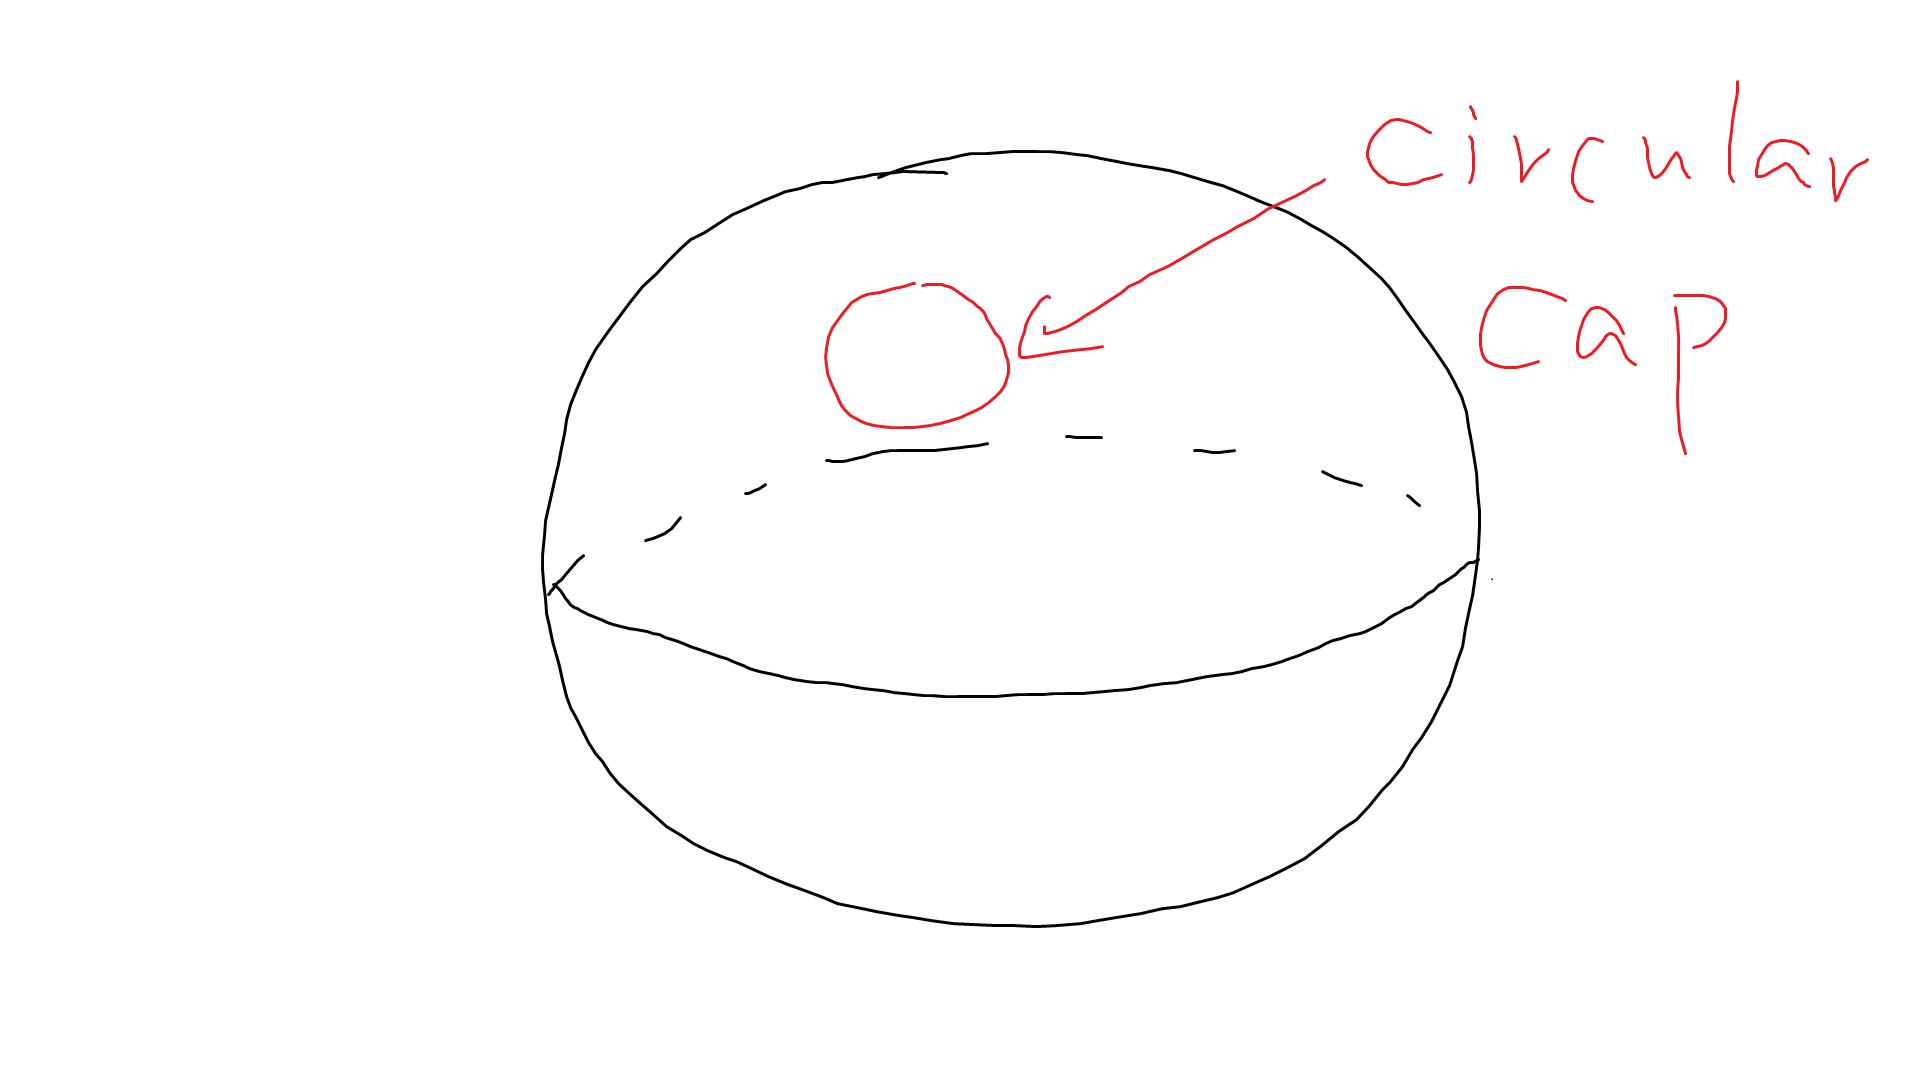
\includegraphics[scale=0.5]{image/Comb_01.png}

For a set $A$ of vertices in a graph $G$, the \emph{boundary} of $A$ is $b(A) = \{x\in V(G): x \not\in A, xy \in E$ for some $y \in A\}$.\\
e.g. in diagram
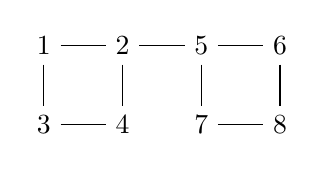
\begin{tikzpicture}
    \node (1) at (0,0) {1};
    \node (2) at (1,0) {2};
    \node (3) at (0,-1) {3};
    \node (4) at (1,-1) {4};
    \node (5) at (2,0) {5};
    \node (6) at (3,0) {6};
    \node (7) at (2,-1) {7};
    \node (8) at (3,-1) {8};

    \path (1) edge (2);
    \path (1) edge (3);
    \path (2) edge (4);
    \path (3) edge (4);
    \path (2) edge (5);
    \path (5) edge (6);
    \path (5) edge (7);
    \path (6) edge (8);
    \path (7) edge (8);
\end{tikzpicture}
, if $A = \{1,2,3\}$, then $b(A) = \{4,5\}$.

An \emph{isoperimetric inequality} of $G$ is an inequality of form: $|B(A)| \geq f(|A|) \forall A \subset V(G)$.\\
Equivalently, minimise the \emph{neighbourhood} of $A$: $N(A) = A \cup b(A) = \{x \in G: d(x,A) \leq 1\}$.\\
A natural guess is often $B(x,r) = \{y \in G: d(x,y) \leq r\}$.\\
What happens in $Q_n$? e.g. $|A| = 4$ in $Q_3$, take all vertices with at least one component 0, then $|b(A)| = 3$; if we instead take all vertices in the lower half plane then $|b(A)| = 4$.

Our guess: \emph{balls are best}, i.e. if $|A| = |X^{(\leq r)}|$, then $|N(A)| \geq |X^{(\leq r+1)}|$ (obvious notations).\\
What if $|A|$ is strictly between $\sum_{i=0}^r {n \choose i}$ and $\sum_{i=0}^{r+1} {n \choose i}$?\\
We guess that $A=X^{(\leq r)} \cup B$ for some $B \subset X^{(r+1)}$ (this is called a \emph{hamming ball}).\\
If we knew this, then $N(A) = X^{(\leq r+1)} \cup \partial^+ B$; hence in this case we know which $B$ to take -- by K-K theorem, take $B$ to be an initial segment of \emph{lex}.

We define the \emph{simplicial} order on $Q_n$ by $x<y$ if either $|x| < |y|$ or $|x|=|y|$ and $x<y$ in lex.\\
Our aim then becomes proving that initial segments of simplicial are best.\\

Given $A \subset Q_n$, and $1 \leq i \leq n$, the \emph{$i$-section} are the set systems $A^{(i)}_+, A^{(i)}_- \subset \P(X-i)$ (\emph{$Q_{n-1}$}), given by
$$A^{(i)}_- = \{x \in A:i \not\in X \} \subset \P(X-i)$$
$$A^{(i)}_+ = \{x -\{i\}: x \in A, i \in x\} \subset \P(X-i)$$
(the first is taking all elements of $A$ that don't contain $i$, the second is taking all elements of $A$ that have $i$ and then throw $i$ away and keep the result).

Define the \emph{$i$-compression} $C_i(A)$ of $A$ by giving its $i$-sections:\\
$C_i(A)^{(i)}_+ =$ initial segment of $Q_{n-1}$ of size $|A^{(i)}_+|$;
$C_i(A)^{(i)}_- =$ initial segment of $Q_{n-1}$ of size $|A^{(i)}_-|$;

Certainly, $|C_i(A)| = |A|$. Also, $C_i(A)$ \emph{looks more like} an initial segment of simplicial than $A$ did. We say $A$ is \emph{$i$-compressed} if $C_i(A) = A$.

\begin{thm} (1, Harper\footnote{Harper first gave a proof with a \emph{lot} of holes inside with no one knowing how to fill those...}'s)\\
    Let $A \subset Q_n$, and let $C$ be the initial segment of simplicial order with $|C| = |A|$. Then $|N(A)| \geq |N(C)|$.\\
    In particular, if $|A| \geq \sum_{i=0}^r {n \choose i}$, then $|N(A)| \geq \sum_{i=0}^{r+1} {n \choose i}$.

    \begin{rem}
        $\bullet$ If we know $A$ is a Hamming ball then we're done by K-K theorem;\\
        $\bullet$ Harper implies K-K trivially: given $B \subset X^{(r)}$, just apply Harper to $A=B \cup X^{(\leq r-1)}$.
    \end{rem}
    
    \begin{proof}
        Induction on $n$. $n=1$ is trivial.\\
        Given $A \subset Q_n(n>1)$: fix $1 \leq i \leq n$. We claim that $|N(C_i(A))| \leq |N(A)|$.\\
        Proof of claim: write $B = C_i(A)$. We have $|N(A)| = |A_+ \cup N(A_-)| + |A_- \cup N(A_+)|$ (downstairs and upstairs respectively. Think)\\
        Similarly, $|N(B)| = |B_+ \cup N(B_-)| + |B_- \cup N(B_+)|$.\\
        Now $|B_+| = |A_+|$, and $|N(B_-)| \leq |N(A_-)|$ (induction). But $N(B_-)$ is an initial segment of simplicial (on $Q_{n-1}$), as is $B_+$, so $N(B_-)$ and $B_+$ are \emph{nested} (i.e. one belongs to another).\\
        Hence $|B_+ \cup N(B_-)| \leq |A_+ \cup N(A_-)|$.\\
        Similarly, $|B_- \cup N(B_+)| \leq |A_- \cup N(A_+)|$. Thus $|N(B)| \leq |N(A)|$.\\

        ---Lecture 8---

        Among all $B \subset Q_n$ with $|B| = |A|$ and $|N(B)| \leq |N(A)|$, choose one with $\sum_{x \in B} f(x)$ minimal where $f(x)$ is the position of $x$ in simplicial order on $Q_n$. Then $B$ is $i$-compressed $\forall i$.\\
        Must such $A,B$ be an initial segment of simplicial? Unfortunately the answer is no, e.g. take $A=\{\phi,1,2,12\} \subset Q_3$.
        However we have 
        \begin{lemma} (2)\\
            Let $B \subset Q_n$ be $i$-compressed for all $i$, but not an initial segment of the simplicial order. Then\\
            $\bullet$ If $n=2k+1$ is odd, we have $B=X^{(\leq k)} - (k+2)(k+3)...(2k)(2k+1) \cup 12...k(k+1)$, i.e. removing the last element in $X^{(k)}$ but add in the first element in $X^{(k+1)}$;\\
            $\bullet$ If $n=2k$ is even, we have $B=X^{(\leq k-1)} \cup \{x \in X^{(k)}: 1 \in x\} - 1(k+2)(k+3)...(2k) \cup 234...k(k+1)$, i.e. cut exactly half in the middle layer but removing the last element with 1 and add in the first element without 1.

            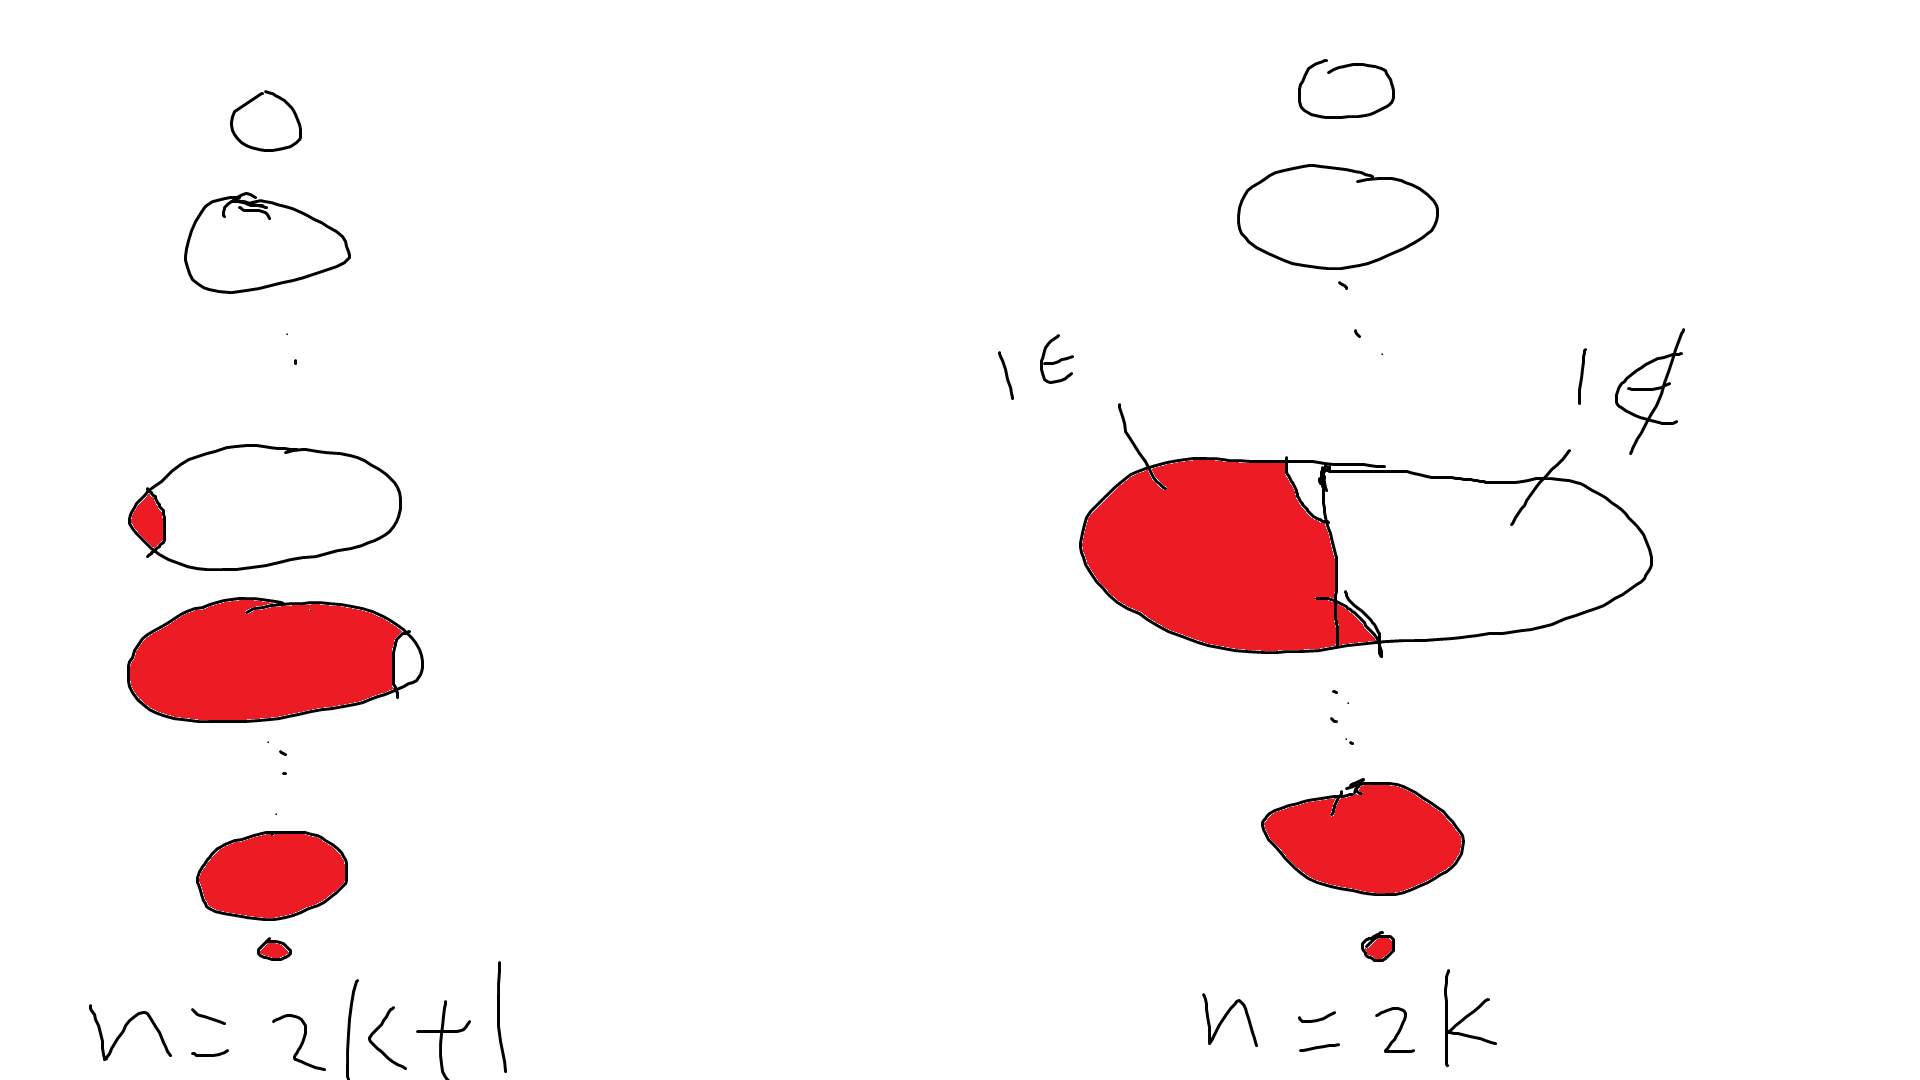
\includegraphics[scale=0.5]{image/Comb_02.png}

            Note that this is trivially beaten by the initial segment of the same size -- so we can prove Harper's theorem if we could prove this.
            \begin{proof}
                Suppose we have $x \not\in B, y \in B$ for some $x,y$ with $x<y$ in simplicial order. Note that we cannot have $i \in x, i \in y$ (as $B$ is $i$-compressed) for any $i$; similarly we cannot have $i \not\in x, i \not\in y$. So $x$ and $y$ must be complement to each other.\\
                Hence for each $y \in B$, at most one $x<y$ has $x \not\in B$ (namely $y^c$); and for each $x\not\in B$ at most one $y>x$ ahs $y \in B$ ($x^c$). Hence $B=\{z:z \leq y\} - \{x\}$, where $x$ is the immediate predecessor of $y$ and $x=y^c$. But then $x$ is the last $k$-set (if $n=2k+1$) or the last $k$-set containing 1 (if $n=2k$).
            \end{proof}
        \end{lemma}
    \end{proof}
\end{thm}

\begin{rem}
    1. We can also prove this by $UV$-compressions.\\
    2. We can also use these \emph{codimension-1} compression to prove K-K theorem directly.
\end{rem}

Now there's no reason to consider only the neighbourhood within one step. For $A \subset Q_n$, the \emph{$t$-neighbourhood} of $A$ is $A_{(t)} = N^t (A) = \{x \in Q_n: d(x,A) \leq t\}$.

\begin{coro} (3)\\
    Let $A \subset Q_n$ with $|A| = |X^{(\leq r)}|$. Then, for $1 \leq t \leq n-r$, we have $|A_{(t)}| \geq |X^{(\leq r+t)}|$.
    \begin{proof}
        Apply Harper's theorem and use induction.
    \end{proof}
\end{coro}

To get a feel for what corollary 3 is saying, we'll need some estimates on things like $\sum_{i=0}^r {n\choose i}$. Note that this is essentially just estimating $\P(X<=r)$ where $X \sim B(n,\frac{1}{2})$. So by CLT we could just use normal distribution to get an accurate estimate when $n$ is large.\\
Lecturer decided to still write a proposition down in the end.

\begin{prop} (4)\\
    Let $0 < \varepsilon < \frac{1}{4}$, Then for $r=\lfloor \frac{1}{2} -\varepsilon/n\rfloor$, the above sum (let's use $S$ to denote that) is at most $\frac{1}{\varepsilon} e^{-\varepsilon^2 n/2} 2^n$ (an exponentially small fraction of $2^n$, with $\varepsilon$ fixed).\\
    \begin{proof}
        For $i \leq (\frac{1}{2} - \varepsilon) n$:
        \begin{equation*}
            \begin{aligned}
                \frac{{n \choose {i-1}}}{{n \choose i}} &= \frac{i}{n-i+1} \leq \frac{\frac{1}{2}-\varepsilon}{\frac{1}{2}+\varepsilon}\\
                &= 1-\frac{2\varepsilon}{\frac{1}{2}+\varepsilon}\\
                &\leq 1-2\varepsilon
            \end{aligned}
        \end{equation*}
        Hence $S \leq \frac{1}{2\varepsilon}{n \choose {\lfloor (\frac{1}{2}-\varepsilon) n \rfloor}}$.\\
        Similarly we could estimate (note we have to be careful about the floor sign)
        \begin{equation*}
            \begin{aligned}
                {n \choose {\lfloor (\frac{1}{2}-\varepsilon) n \rfloor}} &\leq (1-\varepsilon)^{\varepsilon n/2-1} {n \choose {\lfloor (\frac{1}{2}-\frac{\varepsilon}{2}) n \rfloor}}\\
                &\leq 2(1-\varepsilon)^{\varepsilon n/2} 2^n\\
                &\leq 2 e^{-\varepsilon \cdot \varepsilon n/2} \cdot 2^n
            \end{aligned}
        \end{equation*}
        Thus $S \leq \frac{1}{2\varepsilon} 2e^{-\varepsilon^2 n/2} 2^n$.
    \end{proof}
\end{prop}

---Lecture 9---

\begin{thm} (5)\\
    Let $A \subset Q_n$ with $\frac{|A|}{2^n} \geq 1/2$, and $0 < \varepsilon < 1/4$. Then
    $$\frac{|A_{(\varepsilon_n)}|}{2^n} \geq 1-\frac{2}{\varepsilon} e^{-\varepsilon^2 n/2}$$
    (Slogan: \emph{1/2-sized sets have exponentially large $\varepsilon n-$neighbourhood}.)
    \begin{proof}
        It's enough to show that if $\varepsilon_n$ is an integer then the above holds.\\
        We have $|A| \geq \sum_{i=0}^{\lceil n/2-1\rceil} {n\choose i}$ (if $n$ is even this is trivial, if $n$ is odd this is exactly halfway). So by Harper's, we have
        $$|A_{(\varepsilon_n)}| \geq \sum_{i=0}^{\lceil n(1/2+\varepsilon)-1\rceil} {n \choose i}$$
        i.e. 
        $$|A_{(\varepsilon_n)}^c| \leq \sum_{i=\lceil n(1/2+\varepsilon)\rceil}^n {n \choose i} = \sum_{i=0}^{\lfloor n(1/2-\varepsilon)\rfloor} {n \choose i} \leq \frac{1}{\varepsilon} e^{-\varepsilon^2 n/2} \cdot 2^n$$

    \end{proof}
\end{thm}

\subsection{Concentration of Measure}

Say $f:Q_n \to \R$ is \emph{Lipschitz} if $|f(x)-f(y)| \leq 1$ $\forall x,y \in Q_n$ adjacent (see part IB Analysis II for the original meaning).\\
We say $M \in \R$ is a \emph{median} or \emph{L\'evy mean} of $f$ if $|\{x:f(x) \leq M\}|$, $|\{x:f(x) \geq M\}| \geq \frac{1}{2}\cdot 2^n$.\\
Now we are ready to show \emph{every well-behaved function on $Q_n$ is roughly constant nearly everywhere}.

\begin{thm} (6)\\
    Let $f:Q_n \to \R$ be Lipschitz, with median $M$, and $0<\varepsilon<\frac{1}{4}$. Then
    $$\frac{|\{x:|f(x)-M| \leq \varepsilon n\}|}{2^n} \geq 1-\frac{4}{\varepsilon} e^{-\varepsilon^2 n/2}$$
    \begin{proof}
        Let $A=\{x:f(x) \leq M\}$.\\
        Then $\frac{|A|}{2^n} \geq \frac{1}{2}$. So $\frac{|A_{(\varepsilon n)}|}{2^n} \geq 1-\frac{2}{\varepsilon} e^{-\varepsilon^2 n/2}$.\\
        However, $x \in A_{(\varepsilon_n)} \implies f(x) \leq M+\varepsilon n$ as $f$ is Lipschitz. So 
        $$\frac{|\{x:f(x) \leq M+\varepsilon n\}|}{2^n} \geq 1-\frac{2}{\varepsilon} e^{-\varepsilon^2 n/2}$$
        Same argument shows that
        $$\frac{|\{x:f(x) \geq M-\varepsilon n\}|}{2^n} \geq 1-\frac{2}{\varepsilon} e^{-\varepsilon^2 n/2}$$
        Intersect with and we get the desired result.
    \end{proof}
    This is sometimes called the \emph{concentration of measure phenomenon}.
\end{thm}

Let $G$ be a graph of diameter $D$. Let
$$\alpha(G,\varepsilon) = \max\{1-\frac{|A_{(\varepsilon D)}|}{|G|}: A \subset G, \frac{|A|}{|G|} \geq \frac{1}{2}\}$$
So $\alpha(G,\varepsilon)$ is \emph{small} says \emph{$\frac{1}{2}$-sized sets have big $\varepsilon D$-neighbourhoods}.\\
We say a sequence of graphs $G_1,G_2,...$ is a \emph{L\'evy family} if $\alpha(G_n,\varepsilon) \to 0$ as $n \to \infty$ (for each fixed $\varepsilon$).\\
Thus theorem 5 says: $Q_1,Q_2,Q_3,...$ forms a L\'evy family (even a \emph{normal} one, i.e. $\alpha(G_n,\varepsilon)$ is exponentially small in $A$ for each fixed $\varepsilon$).\\
So we have concentration of measure (as in theorem 6 for any L\'evy family).\\
Many natural families of graphs form L\'evy families, e.g. symmetric group $S_n$ (made into a graph by joining $x,y$ if $xy^{-1}$ is a transposition).

Similarly, we can define $\alpha(X,\varepsilon)$ for $x$ any metric measure space (of finite diameter and finite measure) -- so again we have concentration of measure for any L\'evy family.\\

\begin{eg}
    Consider the sphere $S^n \subset \R^{n+1}$ (note that $D=1$ so we can omit it in this example).\\
    To show \emph{all 1/2-sized sets have big $\varepsilon$-neighbourhoods}, we need 2 ingredients:\\
    (1) An isoperimetric inequality: if $A \subset S^n$ and $C \subset S^n$ is the circular cap of the same size ($|C| = |A|$), then $|A_{(\varepsilon)}|\geq |C_{(\varepsilon)}|$.\\
    To prove this we'd like to have some way to \emph{compress} $A$ into something that is more like $C$, while reducing (at least not increasing) it's $\varepsilon$-neighbourhood. One way is to \emph{stamp on your set}, i.e. always move point \emph{above} equator to corresponding point \emph{below} the equator, if possible.

    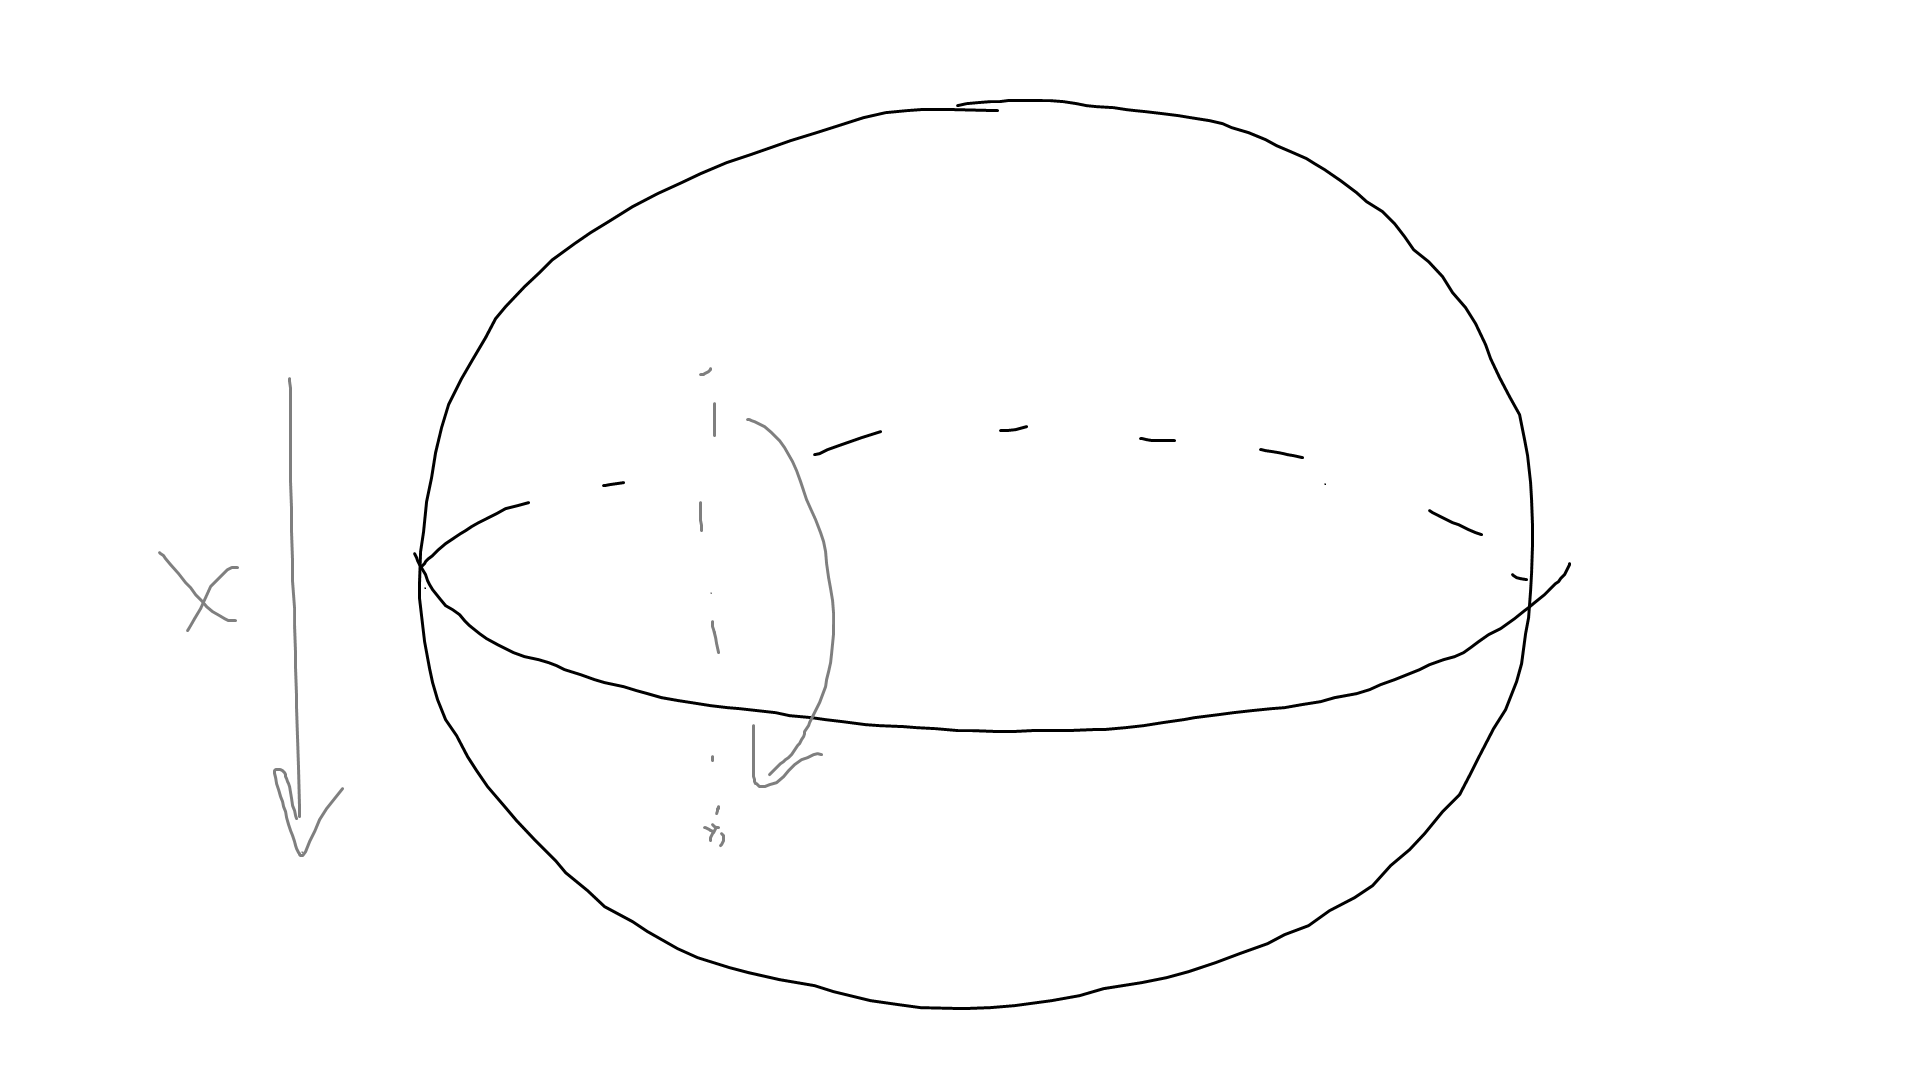
\includegraphics[scale=0.5]{image/Comb_03.png}

    But note that we can choose any direction for the compression. Then by some arguments we could prove that $A$ converges to a circular cap.\\
    The above compression is sometimes called \emph{2-point symmetrisation}.\\
    (2) An estimate: let $C$ be circular cap with $|C| = \frac{1}{2}$, i.e. with angle $\frac{\pi}{2}$ (so exactly half the surface of a sphere). Then $C_{(\varepsilon)}$ is the circular cap of angle $\frac{\pi}{2}+\varepsilon$.\\
    However, we know from common sense that almost all of the surface area concentrates around the equator in high dimensions. So $C_{(\varepsilon)}$ is indeed big.\\
    (More rigourously, the remaining volume is approximately $\int_\varepsilon^{\frac{\pi}{2}} (\cos \theta)^n d\theta$ which tends to $0$ exponentially fast as $n \to \infty$ for any fixed $\varepsilon>0$).
\end{eg}

---Lecture 10---

We deduced concentration of measure from isoperimetric estimates conversely:

\begin{prop}
    Let $G$ be a graph s.t. for any Lipschitz $f:G \to \R$ with median $M$ we have 
    $$\frac{|\{x \in G:|f(x)-M| \leq t\}|}{|G|} \geq 1-\alpha$$
    (for some given $t,\alpha$). Then for $A \subset G$ with $\frac{|A|}{|G|} \geq \frac{1}{2}$ we have $\frac{|A_{(t)}|}{|G|} \geq 1-\alpha$.
    \begin{proof}
        The function $f(x) = d(x,A)$ is Lipschitz and has $0$ as a median (as $|A| \geq \frac{1}{2}|G|$).
    \end{proof}
\end{prop}

\subsection{Edge-isoperimetric inequalities}

For $A \subset G$ ($G$ a graph), the \emph{edge-boundary} of $A$ is $\partial A = \{xy \in E(G): x \in A, y \not\in A\}$.

For example, in

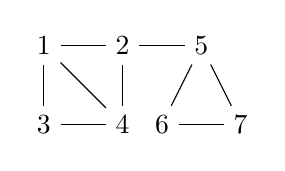
\begin{tikzpicture}
    \node (1) at (0,0) {1};
    \node (2) at (1,0) {2};
    \node (3) at (0,-1) {3};
    \node (4) at (1,-1) {4};
    \node (5) at (2,0) {5};
    \node (6) at (1.5,-1) {6};
    \node (7) at (2.5,-1) {7};

    \path (1) edge (2);
    \path (1) edge (3);
    \path (2) edge (4);
    \path (3) edge (4);
    \path (1) edge (4);
    \path (2) edge (5);
    \path (5) edge (6);
    \path (5) edge (7);
    \path (6) edge (7);
\end{tikzpicture}

the set $A=1,3,4$ has $|\partial A|=2$ ($12,14$). 

For another example, suppose $|A|=4$ and we work in $Q_3$. If we choose $A=\phi,1,2,3$ then $|\partial A| = 6$; however if we use $A=\phi,1,2,12$ then $|\partial A| = 4$.\\
This suggests that, perhaps subcubes are best (instead of simplicial). What if $2^k < |A| < 2^{k+1}$?

We define yet another ordering on $Q_n$: say $x<y$ in the \emph{binary} ordering on $Q_n$ if $\max(x \triangle y) \in y$. Equivalently, $x<y$ if $\sum_{i \in x} 2^i < \sum_{i \in y} 2^i$ (i.e. treat them as binary numbers).

Our aim is to prove that initial segments of binary are best for $\partial A$ in this problem.\\
In particular, $|A|=2^k \implies |\partial A| = 2^k (n-k)$ (each point has $n$ directions; $k$ are inside $A$, so each point sends $n-k$ outside).

For $A \subset Q_n$ and $1 \leq i \leq n$, the \emph{$i$-binary compression} $B_i(A)$ is defined by giving its $i$-sections:\\
$B_i(A)^{(i)}_+ = $ first $|A^{(i)}_+|$ elements of $\P(X-i)$ in binary,\\
$B_i(A)^{(i)}_- = $ first $|A^{(i)}_-|$ elements of $\P(X-i)$ in binary (we defined these two $A$ sets previously when we proved Harper's theorem).

Note that $|B_i(A)| = |A|$. We say $A$ is $i$-binary-compressed if $B_i(A) = A$.

\begin{thm} (8, edge-isoperimetric inequality in the cube\footnote{This is sometimes called Harper-Lindsey-Berstein-Hart theorem. Basically Harper gave another proof with lots of holes, Bernstein tried to fix them but he missed some of them, and Hart fixed the proof in the end. Meanwhile Lindsey gave a generalized version of the theorem (which is correct).})\\
    Let $A \subset Q_n$, and let $C$ be the initial segment of the binary ordering with $|C| = |A|$. Then $|\partial A| \geq |\partial C|$.\\
    In particular, if $|A| = 2^k$ then $|\partial A| \geq 2^k (n-k)$.
    \begin{proof}
        Induction on $n$: $n=1$ is trivial.\\
        Given $A \subset Q_n$ $(n>1)$, and $1 \leq i \leq n$, we claim $|\partial B_i(A)| \leq |\partial A|$: to prove that, write $B$ for $B_i(A)$.\\
        We have $|\partial A| = |\partial (A_-)| + |\partial (A_+)| + |A_- \triangle A_+|$ (which are downstairs, upstirs, and in direction $i$ respectively);\\
        Also $|\partial B| = |\partial(B_-)| + |\partial(B_+)| + |B_- \triangle B_+|$.\\
        Now we have $|\partial(B_-)| \leq |\partial(A_-)|$ and $|\partial(B_+)| \leq |\partial (A_+)|$ (induction).\\
        Also, $|A_-| = |B_-|$, $|A_+|=|B_+|$, and $B_-,B_+$ are nested (i.e. one a subset of another). So by triangle inequality we're done with the claim.\\

        Back to main proof: among all $B\subset Q_n$ with $|B| = |A|$ and $|\partial B| \leq |\partial A|$, choose one with $\sum_{x\in B}($position of $x$ in binary order$)$ minimal (note that position of $x$ in binary order is just the binary number it corresponds to).\\
        Then $B$ is $i$-binary-compressed for all $i$ (by claim). Unfortunately this $B$ need not be an initial segment of binary -- e.g. $B=\{\phi,1,2,3\}$.\\
        However this is also the only counterexample -- we claim that if $B$ is $i$-binary-compressed for all $i$ but not an initial segment of binary, then it has to be $\P(n-1) \cup n - 123...(n-1)$, i.e. the \emph{bottom-half} of the cube, with last point replaced by the first point of top half. Then we are done as this is clearly worse than the bottom half of the cube.\\
        To prove the claim, suppose we have some $x<y$ with $x \not\in B$ but $y\in B$. Then forall $i$ we cannot have $i \not\in x,y$, nor $i \in x,y$ (as $B$ is $i$-compressed). This holds for all $i$, so $x=y^c$.\\
        Thus for each $y \in B$, there is at most one $x<y$ with $x \not\in B$ (its complement); for each $y \not\in B$, there is at most 1 $y>x$ that is in $B$. But then $x$ and $y$ must be consecutive in the binary order, therefore the result.
    \end{proof}
\end{thm}

\begin{rem}
    In both of these theorems (1 and 8, for vertices and edges respectively), it was vital that the extremal sets in dimension $n-1$ were nested, i.e. they were the initial segments of some ordering.
\end{rem}

---Lecture 11---

Final lecture is on Thursday 9am 29th Nov.

Example class on Friday 23rd 4pm.

Define the \emph{isoperimetric number} of a graph $G$ is $i(G) = \min\{\frac{|\partial A|}{|A|}: A \subset G, |A| \leq \frac{1}{2}|G|\}$.\\
Slogan: \emph{How small can the average out-degree be}?

\begin{coro}
    $i(Q_n) = 1$.
    \begin{proof}
        The set $A = \P([n-1])$ shows $i(Q_n) \leq 1$.\\
        To show the other inequality, it's sufficient to show (by theorem 8) that if $C$ is an initial segment of binary with $|C| \leq 2^{n-1}$, then $|\partial C| \geq |C|$.
            But this is clear because $C \subset \P([n-1])$.
    \end{proof}
\end{coro}

\subsection{Inequalities in the grid}

The \emph{grid} is the graph on vertex-set $[k]^n = \{1,2,...,k\}^n$ in which $(x_1...x_n)$ is joind to $(y_1...y_n)$ if for some $i$, we have $|x_i - y_i| = 1$ and $x_j = y_j$ $\forall j \neq i$ (i.e. has $L_1$-distance 1).\\
For $k=2$, this is the discrete cube $Q_n$. Do theorem 1 and theorem 8 have analogues in $[k]^n$?

For best vertex-boundary? e.g. consider $[k]^2$. A natural choice is an $L_1$-ball, but where should we put it? Obviously it's better to put it at the corner instead of in the center of grid. If we use a $L_1$-ball centered at a corner of the grid with radius $d$, then size of the boundary of $A$, $|b(A)| \approx d \approx \sqrt{2|A|}$; if we instead consider a $L_\infty$ ball at the same location, we have $|b(A)| \approx 2d \approx 2\sqrt{|A|}$.\\
This suggests that sets of the form $\{x: |x| \leq r\}$ are best. How about in between? Let's look at some (3d)-diagram:

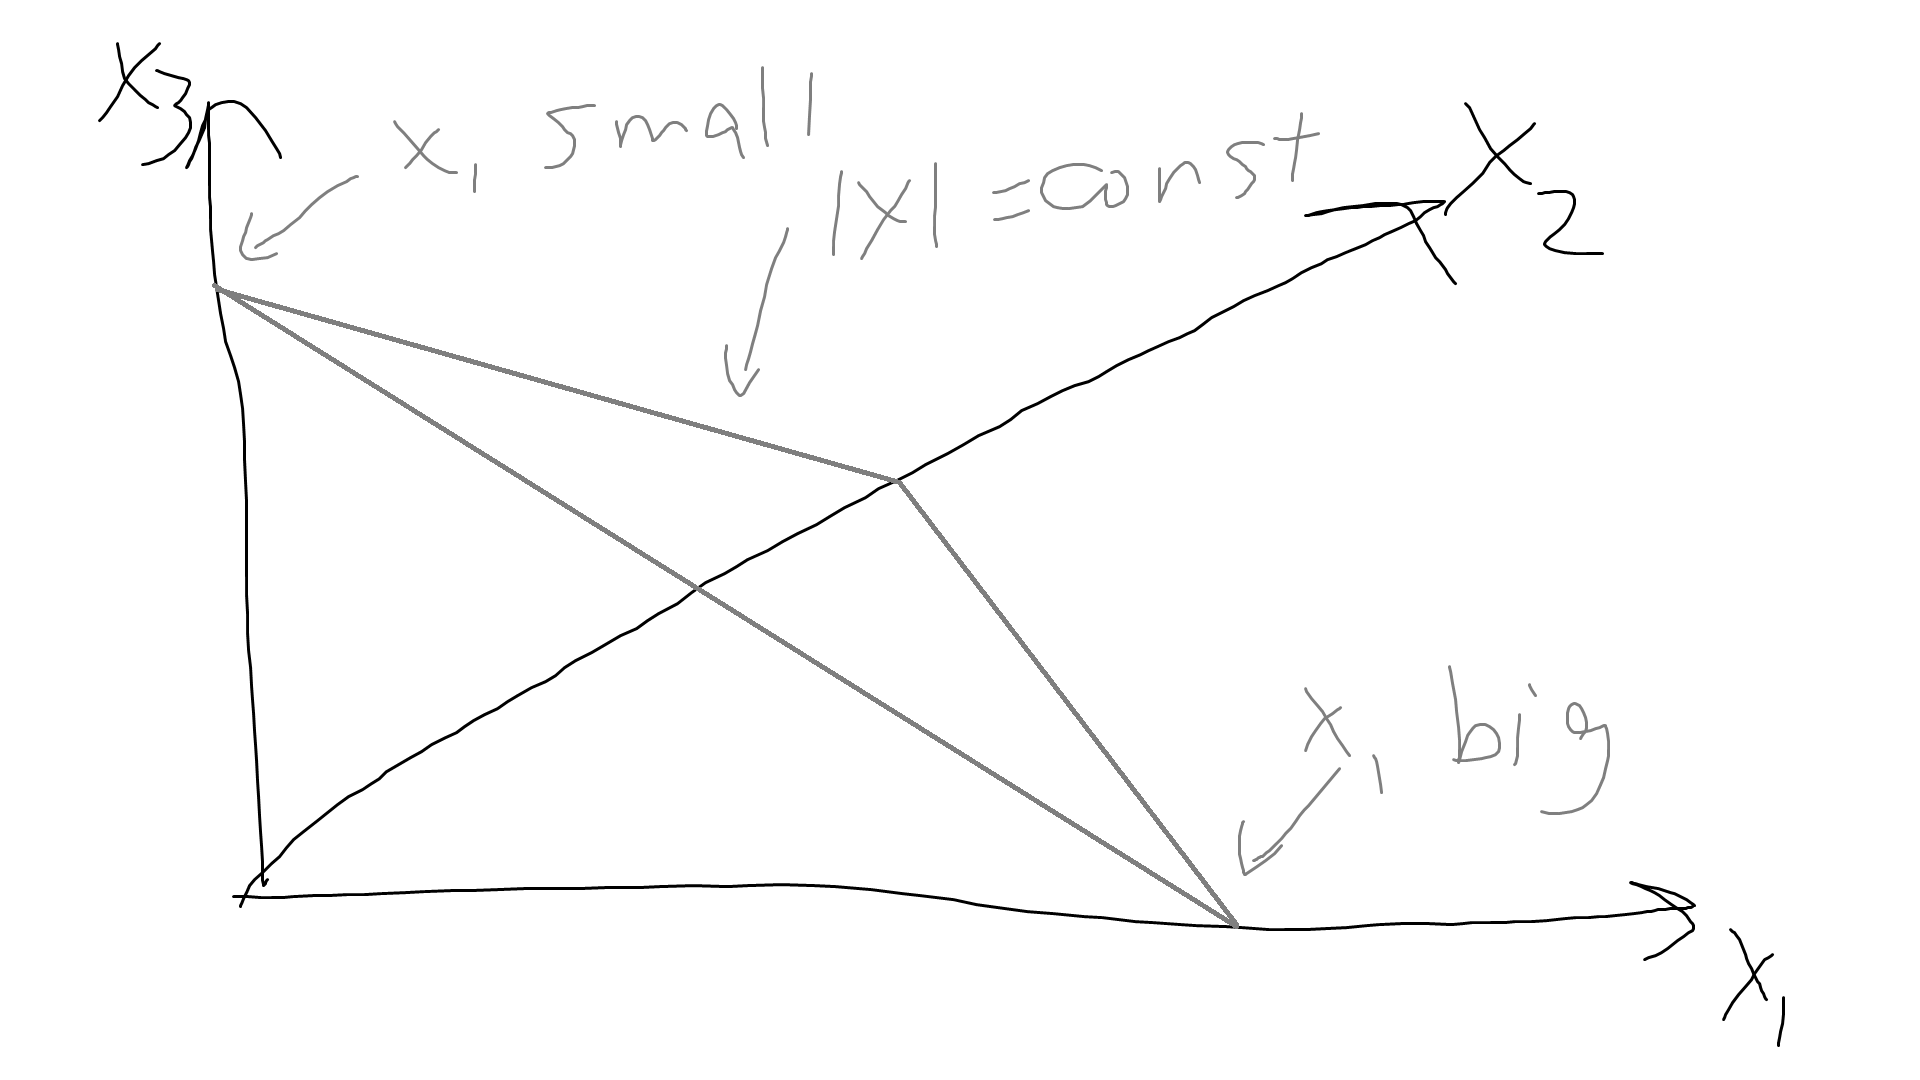
\includegraphics[scale=0.5]{image/Comb_04.png}

For given $|x|$, we'd \emph{keep $x_1$ big}, or more precisely, define the \emph{simplicial ordering} on $[k]^n$ by setting $x<y$ if \emph{either} $|x| < |y|$ or $|x| = |y|$ and $x_i > y_i$ where $i = \min\{j:x_j \neq y_j\}$.\\
Note: for $k=2$, this agrees with the previous definition.

(Some examples)

Obviously, our aim is to show that initial segments of simplicial minimise the neighbourhood.\\
In particular, $|A| = |\{x:|x| \leq r\}| \implies |n(A)| \geq |\{x:|x|\leq r+1\}|$.

For $A \subset [k]^n$ and $1 \leq i\ \leq n$, the \emph{$i$-section} of $A$ are the sets $A_1,...,A_k$ or $A_1^{(i)},...,A_k^{(i)}$ in $[k]^{n-1}$, given by\footnote{Lecturer has $x_n$ as the last term in the expression, but that doesn't really make sense here.}:\\
$$A_t = \{(x_1,...,x_{n-1}) \in [k]^{n-1}: (x_1,x_2,...,x_{i-1},t,x_{i+1},...,x_{n-1}) \in  A\}\ 1 \leq t \leq k$$

The \emph{$i$-compression} $C_i(A) \subset [k]^n$ is defined by giving its $i$-sections:\\
$C_i(A)_t =$ first $|A_t|$ points in simplicial order on $[k]^{n-1}$ (for each $1 \leq t \leq k$).

Certainly $|C_i(A)| = |A|$ (check).\\
We say A is \emph{$i$-compressed} if $C_i(A) = A$.

\begin{thm} (10, vertex-isoperimetric inequality in the grid)\\
    Let $A \subset [k]^n$, and let $C$ be the initial segment of the simplicial order on $[k]^n$ with $|C|=|A|$. Then $|N(A)| \geq |N(C)|$.\\
    In particular, if $|A| \geq |\{x:|x| \leq r\}|$, then $|N(A)| \geq |\{x:|x| \leq r+1\}|$.
    \begin{proof}
        Induction on $n$; $n=1$ is trivial (just one straight line).\\
        Now given $A \subset [k]^n$ ($n>1$), and $1 \leq i\ \leq n$. We claim that $|N(C_i(A))| \leq |N(A)|$: Let $B = C_i(A)$. For $1 \leq t \leq k$, $N(A)_t = N(A_t) \cup A_{t-1} \cup A_{t+1}$ (which are from level $t$, from below and from above respectively, and define $A_0 = A_{k+1} = \phi$).\\
        Similarly, $N(B)_t = N(B_t) \cup B_{t-1} \cup B_{t+1}$. We're again showing $B$ is better than $A$, but the three unions in expression of $N(b)_t$ are nested since they are all initial segment of simplical; also $|B_{t-1}| = |A_{t-1}|$, $|B_{t+1}| = |A_{t+1}|$, and by induction hypothesis $|N(B_t)| \leq |N(A_t)|$. So $|N(B)_t| \leq |N(A)_t|$.\\
        This works for every $1 \leq t \leq k$.\\
        Among all $B \subset [k]^n$ with $|B| = |A|$, and $|N(B)| \leq |N(A)|$, choose one with minimal $\sum_{x \in B} ($ position of $x$ in simplicial$)$.\\
        Then $B$ is $i$-compressed for all $i$ (else $C_i(B)$ contradicts our choice of $B$).\\
        Similarly we are not done -- but we'll left this to next lecture.

        ---Lecture 12---
        
        Example Class 2: Friday 23rd, MR3, 4pm; hand in Q4 and Q6 (on lecture next thursday).

        Now we want to prove that $N(B) \geq N(C)$.\\
        Case 1: $n=2$. Now $B$ is $i$-compressed $\forall i$ iff $B$ is a \emph{down-set}, i.e. if $x_i \leq y_i$ and $y \in B$, then $x \in B$ (\emph{going down or left, we stay in $B$}).\\
        Now suppose $B \neq C$. Let $r = \min\{|x|:x \not\in B\}$, $s = \max\{|x|: x \in B\}$. We must have $r \leq s$, since $r>s \implies B=C$.\\
        $\bullet$ If $r=s$: We have $\{x:|x| \leq r-1\} \subset B \subset \{x:|x| \leq r\}$. But in that case it's trivial that the best we can do to place those points in level $r$ is putting them adjacent at an edge (which is what $C$ does), so $|N(B)| \geq |N(C)|$;\\
        If $r<s$: we cannot have $\{x:|x| = r\}$ disjoint from $B$ (as there's a point in level $s$ and $B$ is a down-set). And similarly, we cannot have $\{x:|x| = s\} \subset B$ (as $B$ is a down-set and $\exists x \not\in B, |x|=r$).\\
        So we have two adjacent (in the sense of they differ by $(1,-1)$) points in level $r$, $x,x'$, such that $x \not\in B$ but $x' \in B$; similarly we have two adjacent $y,y'$ in level $s$ s.t. $y\in B$ but $y' \not\in B$. Now consider $B'=B \cup \{x\} - \{y\}$. This doesn't increase the size of neighbourhood; but this contradicts the choice of $B$.\\
        Case 2: $n \geq 3$. If $x \in B$, then we must have $x-l_n+l_i \in B$ (for any $1 \leq i \leq n-1, x_n >1, x_i<k$) (here $l_i$ referring to the unit vector in $i^{th}$ direction). Because $B$ is $j$-compressed for any $j \neq n,i$ (note that this exists since $n \geq 3$), we have $N(B_t) \subset B_{t-1}$.\\
        We had $N(B)_t = N(B_t) \cup B_{t-1} \cup B_{t+1}$, so $N(B)_t = B_{t-1}$. Thus $|N(B)| = |B_{k-1}| + |B_{k-2}| + ... + |B_1| + |N(B_1)| = |B|-|B_k| + |N(B_1)|$.\\
        Similary, $|N(C)| = |C| - |C_k| + |N(C_1)|$. As a result, it's sufficient to show that $|B_k| \leq |C_k|$ and $|B_1| \geq |C_1|$ (as $C_1$ is the set that minimizes its neighbour among sets of its size in dimension $n-1$).\\
        $\bullet$ $|B_k| \leq |C_k|$: Define $D \subset [k]^n$ by $D_k = B_k$, $D_t = N(D_{t+1})$ ($t=k-1,k-2,...,1$). Then $D$ is an initial segment of simplicial, and $D \subset B$. So $|D| \leq |B| = |C|$; from this we know $D \subset C$ (nested), hence $D_k \subset C_k$.\\
        $\bullet$ $|B_1| \geq |C_1|$: (similar argument) Define $E \subset [k]^n$ by: $E_1 = B_1$, $E_t = \{x \in [k]^{n-1}: N(\{x\}) \subset E_{t-1}\}$, $t=2,3,...,k$. Then $E$ is an initial segment of simplicial; this time $E \supset B$, so $|E| \geq |B| = |C|$ and $E\supset C$. Hence $E_1 \supset C_1$.
    \end{proof}
\end{thm}

\begin{coro} (11)\\
    Let $A \subset [k]^n$ with $|A| = |\{x:|x| \leq r\}|$. Then $|A_{(t)}| \geq |\{x:|x| \leq r+t\}|$.\\
    \begin{proof}
        Induction on $t$.
    \end{proof}
\end{coro}

\begin{rem}
    We can check from this that, for any fixed $k$, the sequence $[k]^1,[k]^2,[k]^3,...$ is a normal L\'evy family.
\end{rem}

\subsection{Edge-isoperimetric inequalities in the grid (\emph{Non-examinable})}

How to minimize $|\partial A|$ in $[k]^n$?\\
For example, in $[k]^2$. If we take the $L_\infty$ ball with radius $d$ then $|\partial A| \approx 2d = 2\sqrt{|A|}$; for the $L_1$ ball with radius $d$, $|\partial A| \approx 2d \approx 2\sqrt{2|A|}$.\\
So (as we would expect) squares do better.

However, let's consider what happens when the size of $A$ increases: when $|A|$ reaches $k^2/4$, we could use a square with side $k/2$, but note that it's equally good to use a column with width $k/4$ at a side. When $|A|$ increases further, if we continuing using the square we get larger $|\partial A|$ then a column would do. The same \emph{phase transition} happens when $|A|$ reaches $3k^2/4$, where everything becomes the complement, and beyond that the complement of a square becomes better.\\
So we realize that the extremal sets are not nested! So we can't use a similar argument, as all of the previous arguments require our extremal sets to be nested.

In $[k]^3$: We similar ahve the transition from $[a]^3$ to $[a]^2 \times [k]$, and later to $[a] \times [k]^2$, then to the complement of a $[a]^2 \times [k]$, and so on (at some sizes that we could easily calculate).\\
Obviously the same happens in higher dimensions. So we can't use compression to solve this problem.\footnote{There is a result for this, but is much harder. (Searching on google reveals that the \href{https://link.springer.com/content/pdf/10.1007/BF01275667.pdf}{result} is actually by the lecturer in 1989!)}

Very few isoperimetric inequalities are known exactly or asymptotically. E.g. the level $X^{(r)}$: $A$ joined to $B$ if $|A \cap B| = r-1$ -- no one can prove anything sharp!

\newpage

\section{Projections}

---Lecture 13---

\emph{If a set has small projections, must it be small?}

Let $A \subset \P(x)$ for $Y \subset X$, the \emph{projection} or \emph{trace} of $A$ on $Y$ is $A|Y = \{x \cap Y:x \in A\}$.\\
For example, if $A=\{14,25,16,127,128\}$, then $A|\{1,2\} = \{1,2,12\}$. We see that $A|Y \subset \P(Y)$.

We say $A$ \emph{covers} or \emph{shatters} $Y$ if $A|Y = \P(Y)$.\\
The \emph{trace number}, or VC(Vapnik-Cervonekis)-dimension of $A$ is $\tr A = \max\{|Y|:A$ shatters $Y\}$.\\
Given $|A|$, how small can $\tr A$ be? Equivalently, if $\tr A < k$, how large can $A$ be? ($A$ doesn not shatter any $k$-set).

Trivially, we must have $|A| \leq (1-\frac{1}{2^k}) 2^n$, else $A$ shatters \emph{every} $k$-set.

We could take $A=X^{(k)}$ -- no $k$-set $Y$ is shattered, as $Y \not\in A|Y$. Our aim is to prove that this is the best.

\begin{rem}
    This is very striking as from each $k$-projection having size $\leq (1-\frac{1}{2^k}) \cdot$ total, we are getting a very small (polynomial in $n$) bound on $|A|$.
\end{rem}

Idea: it's trivial that $|A| \leq |X^{(k)}|$ if $A$ is a \emph{down-set} (if $x \in A, y \subset x$, then $y \in A$). Indeed, we must have $A \subset X^{(<k)}$, since if $A$ contains a set $X$ with $|X| \geq k$ then $A|X = \P(X)$.\\
So we'll try to make $A$ into a down-set.

For $A \subset \P(X)$, and $1 \leq i \leq n$, the \emph{$i$-down-compression} of $A$ is defined as follows: for $x \in \P(X)$, set 
\begin{equation*}
    \begin{aligned}
        D_i(x) = \left\{\begin{array}{ll}
            x & i \not\in x\\
            x-\{i\} & i \in x
        \end{array}
        \right.
    \end{aligned}
\end{equation*}
and set $D_i(A) = \{D_i(x):x \in A\} \cup \{x \in A: D_i(x) \in A\}$ (remove element $i$ where possible).

\begin{thm} (Sauer-Shelah lemma)\\
    Let $A \subset \P(X)$ with $\tr A < k$. Then $|A| \leq |X^{(k)}|$.
    \begin{proof}
        Given $1 \leq i \leq n$, we claim $\tr(D_i(A)) \leq \tr A$: write $B=D_i(A)$. We'll show that if $B$ shatters $Y$ for some $Y$, then $A$ does as well.\\
        If $i \not\in Y$, then $B|Y = A|Y$, so we may assume $i \in Y$.\\
        Given $z \subset Y$ with $i \not\in z$, we'll show $z, z\cup\{i\} \in A|Y$. Since $z \cup \{i\} \in B|Y$, we have $z \cup \{i\} \cup x \in B$ for some $x \subset X|Y$. Hence $z \cup x$ and $z \cup \{y\} \cup x \in A$ (definition of $D_i$) whence $z,z\cup \{i\} \in A|Y$.\\
        Now let $D=D_n(D_{n-1}(...(D_1(A))))$. Then $|D|=|A|$, $D$ is a down-set, and $\tr D \leq \tr A$.
    \end{proof}
\end{thm}

\begin{rem}
    We used 1-dimensional compressions. We have: if all $k$-dimensional projections have size $\leq 2^k-1$, then $A$ is small ($|A| \leq \sum_{i=0}^{k-1} {n \choose k}$). What about other bounds? For example, what if each $k$-dimensional projection is $\leq 1/2$-sized $(A|Y| \leq 2^{k-1}$)?
\end{rem}

We say a \emph{box} or \emph{brick} in $\R^n$ is a set of the form $[a_1,b_1] \times [a_2,b_2] \times ... \times [a_n, b_n]$ where $a_i \subseteq b_i \forall i$.\\
A \emph{body} $S \subset \R^n$ is a finite union of bricks.\\
Write $|S|$ or $\mu(S)$ for the volume of $S$.

\begin{rem}
    1. Everything unchanged if we only assume $S$ compact (or just bounded and measurable).\\
    2. For $A \subset \P(X) \leftrightarrow \{0,1\}^n$, we have corresponding body $\hat{A} \subset \R^n$ with $\mu(\hat{A}) = |A|$, namely
    $$\hat{A} = \cup_{x \in A} [x_1,x_1+1] \times [x_2,x_2+1] \times ... \times [x_n,x_n+1]$$
\end{rem}

For body $S \subset \R^n$, and $Y \subset \{1,...,n\}$, write $S_Y$ for the projection of $S$ onto the subspace spanned by the basis vectors $e_i,i \in Y$.\\
For example, for $S \subset \R^3$: $S_1$ is the projection of $S$ onto the $x$-axis, i.e. $S_1 = \{x_1:(x_1,x_2,x_3) \in S$ for some $x_2,x_3\}$, and $S_{12}$ is the projection of $S$ onto the xy-plane, i.e. $S_{12} = \{(x_1,x_2):(x_1,x_2,x_3) \in S$ for some $x_3\}$.

Question: do bounds on some of the $|S_Y|$ give bounds on $|S|$?

---Lecture 14---

E.g. for $S \subset \R^3$: $|S| \leq |S_1| |S_2| |S_3|$ -- as $S \subset S_1 \times S_2 \times S_3$;\\
$|S| \leq |S_{12}| |S_3|$ as $S \subset S_{12} \times S_3$.\\
But $|S_{12}|,|S_{13}|$ does not bound $|S|$ -- e.g. $S=[0,\frac{1}{N}] \times [0,N] \times [0,N]$.\\
How about $|S_{12}|,|S_{13}|,|S_{23}|$?

\begin{prop} (2)
    Let $S$ be a body in $\R^3$. Then $|S|^2 \leq |S_{12}||S_{13}||S_{23}|$.

    Notes: 1. we can have eqaulity, e.g. when $S$ is a brick.\\
    2. for $S \subset \R^n$, the \emph{sections} of $S$ are the sets $S(x) \subset \R^{n-1}$ ($x \in \R$) given by $S(x) = \{(x_1...x_{n-1}) \in \R^{n-1}:(x_1...x_{n-1}x) \in S\}$.

    \begin{proof}
        Suppose first that every section of $S$ is a square -- $S(x) =[0,f(x)] \times [0,f(x)]$ $\forall x$. Then $|S_{12}| = M^2$, where $M=\max f$. Also, $|S_{13}| = |S_{23}| = \int f(x) dx$.\\
        So we want $(\int f^2)^2 \leq M^2 (\int f)^2$, i.e $\int f^2 \leq M \int f$, which is true because $f(x)^2 \leq M \cdot f(x)$ $\forall x$.\\
        For general $S$, define body $T \subset \R^3$ by giving its sections:
        $$T(x) = [0,\sqrt{|S(x)|}] \times [0,\sqrt{|S(x)|}]$$
        So $|T| = |S|$.\\
        Certainly we have $|T_{12}| \leq |S_{12}|$ since $|T_{12}| = \max |T(x)|$. Write $g(x) = |S(x)_1|$, $h(x) = |S(x)_2|$, so $|S(x)| \leq g(x)h(x)$.\\
        We have $|S_{13}| = \int g(x) dx$, and $|S_{23}| = \int h(x) dx$. Also, $|T_{13}| = |T_{23}| = \int \sqrt{|S(x)|} dx \leq \int \sqrt{g(x)h(x)} dx$.\\
        So we need $(\int \sqrt{gh})^2 \leq (\int g)(\int h)$, i.e $\int \sqrt{gh} \leq (\int g)^{1/2} (\int h)^{1/2}$ but this is just the Cauchy-Schartz inequality.
    \end{proof}
\end{prop}

Say sets $Y_1 ... Y_r \subset [n]$ \emph{cover} $[n]$ if $Y_1 \cup ... \cup Y_r = [n]$.\\
They are a \emph{$k$-uniform cover} if each $i \in [n]$ belongs to exactly $k$ of $Y_1,...,Y_r$.\\
(Some examples)\\
Our aim is to show that $|S|^k \leq |S_{Y_1}|...|S_{Y_r}|$ when $Y_1,...,Y_r$ is a $k$-uniform cover of $[n]$.\\
Let $\mathcal{C} = \{Y_1,...,Y_k\}$ be a $k$-uniform cover of $[n]$. This is a multiset, i.e. some of the $Y_i$'s could be equal.\\
Now define something that is reminiscent of our previous $i$-sections: $\mathcal{C}_- = \{Y \in \mathcal{C}:n \not\in Y\}$, $\mathcal{C}_+ = \{Y-\{n\} : Y \in \mathcal{C},n \in Y\}$.\\
So $|\mathcal{C}_+| = k$, and $\mathcal{C}_- \cup \mathcal{C}_+$ is a $k$-uniform cover of $[n-1]$.

Note that for a body $S \subset \R^n$: if $n \not\in Y$ then $|S_Y| \geq |S(x)_Y| \forall x$ -- e.g. $|S_1| \geq |S(x)_1| \forall x$ when $S \subset \R^3$.\\
Also, if $n \in Y$, then $|S_Y| = \int |S(x)_{Y-n}| dx$, e.g. $|S_{13}| = \int |S(x)_1| dx$.\\
In proof of proposition 2, we used Cauchy-Schwartz: $\int fg \leq (\int f^2)^{1/2} (\int g^2)^{1/2}$.\\
Here in the general case we'll be using H\"older's inequality: $\int fg \leq (\int f^p)^{1/p} (\int g^q)^{1/q}$, where $\frac{1}{p} + \frac{1}{q} = 1$ (think this was a question on IA Analysis example sheet).\\
Iteration: $\int f_1...f_k \leq (\int f_1^k)^{1/k} ... (\int f_k^k)^{1/k}$.

\begin{thm} (3, uniform cover theorem)\\
    Let $S$ be a body in $\R^n$, and let $\mathcal{C}$ be a $k$-uniform cover of $[n]$. Then $|S|^k \leq \prod_{Y \in \mathcal{C}} |S_Y|$.
    \begin{proof}
        Induction on $n$: $n=1$ is clear.\\
        Given $S \subset \R^n$ where $n>2$,
        \begin{align*}
            |S| &= \int |S(x)| dx\\
            &\leq \int \prod_{Y \in \mathcal{C}_-} |S(x)_Y|^{1/k} \prod_{Y \in \mathcal{C}_+} |S(x)_Y|^{1/k}\\
            &\leq \prod_{Y \in \mathcal{C}_-} |S_Y|^{1/k} \int \prod_{Y \in \mathcal{C}_+} |S(x)_Y|^{1/k}\\
            &\leq \prod_{Y \in \mathcal{C}_-} |S_Y|^{1/k} \prod_{Y \in \mathcal{C}_+} \left(\int |S(x)_Y|\right)^{1/k}\\
            &= \prod_{Y \in \mathcal{C}_-} |S_Y|^{1/k} \prod_{Y \in \mathcal{C}_+} |S_{Y \cup n}|^{1/k}\\
            &= \prod_{Y \in \mathcal{C}} |S_Y|^{1/k}
        \end{align*}
    \end{proof}
\end{thm}

---Lecture 15---

\begin{coro} (4, Loomis-Whitney theorem)\\
    Let $S$ be a body in $\R^n$. Then $|S|^{n-1} \leq \prod_{i=1}^n |S_{[n]-i}|$.
    Note: $n=3$ is proposition 2.
    \begin{proof}
        The sets $[n]-i$, $1 \leq i \leq n$, form an $(n-1)$-uniform cover of $[n]$.
    \end{proof}
\end{coro}

\begin{coro} (5)\\
    Let $A \subset \P([n])$, and let $\mathcal{C}$ be a $k$-uniform cover of $[n]$, then $|A|^k \leq \prod_{Y \in \mathcal{C}} |A|Y|$. In particular, if $|A|Y| \leq (2^{|Y|})^c$ $\forall Y \in \mathcal{C}$, then $|A| \leq (2^n)^c$.
    \begin{proof}
        First part: identify $A$ with body $\hat{A} \subset \R^n$.\\
        Second part: $|A|^k \leq \prod_{Y \in \mathcal{C}} |A|Y| \leq \prod_{Y \in \mathcal{C}} (2^{|Y|})^c = 2^{knc}$.
    \end{proof}
\end{coro}

Our aim is to prove the Bollob\'as-thomason box theorem: for any $S \subset \R^n$, there exsits a box $B$ with $|B| = |S|$ and $|B_Y| \leq |S_Y|$ $\forall Y \subset [n]$. This looks way too strong to be true -- e.g. it tells us that, to verify \emph{any} proposed projection inequality, it suffices to check it on boxes.

A uniform cover $\mathcal{C}$ of $[n]$ is \emph{irreducible} if we cannot write $\mathcal{C} = \mathcal{C}' \cup \mathcal{C}''$ where $\mathcal{C}'$ and $\mathcal{C}''$ are uniform covers.

\begin{lemma} (6)\\
    There are only finitely many irreducible covers of $[n]$.
    \begin{proof}
        Suppose not, let $\mathcal{C}_1,\mathcal{C}_2,...$ are irreducible covers. List $\P([n])$ as $E_1,...,E_{2^n}$. We have subsequence $\mathcal{C}_{i_1},\mathcal{C}_{i_2},...$ on which the number of occurrences of $E_1$ is non-decreasing. Find subsequence of this on which number of occurrences of $E_2$ is non-decreasing, ... Repeating, we get $\mathcal{C}_{j_1},\mathcal{C}_{j_2}$ on which $\forall E \subset [n]$, number of occurrences of $E$ is increasing. But then $\mathcal{C}_{j_2}$ contains $\mathcal{C}_{j_1}$. Contradiction.
    \end{proof}
\end{lemma}

\begin{thm} (7, Bollob\'as-Thomason box theorem)\\
    Let $S \subset \R^n$ be a (non-empty) body. Then there exists a box $B \subset \R^n$ with $|B| = |S|$, and $|B_Y| \leq |S_Y| \forall Y$.
    \begin{proof}
        WLOG let $|S| > 0$ and $n \geq 2$.\\
        Take real variables $x_Y$ for each $Y \subset [n], Y \neq \phi,[n]$.\\
        Consider the inequalities:\\
        $\bullet$ (i) $0 \leq x_Y \leq |S_Y|$ $\forall Y$;\\
        $\bullet$ (ii) $x_Y \leq \prod_{i \in Y} x_i$ for each $|Y| \geq 2$;\\
        $\bullet$ (iii) $|S|^k \leq \prod_{Y \in \mathcal{C}} x_Y$ for each irreducible $k$-uniform cover $\mathcal{C}$ of $[n]$ (for any $k$), apart from $\mathcal{C}=\{[n]\}$.\\
        (We hope to find such $x_Y$ with $|S| = x_1...x_n$ and $x_{12} = x_1x_2$ etc, then our box is $[0,x_1] \times ... \times [0,x_n]$.)\\
        Note that (iii) therefore holds for \emph{all} uniform covers, as it holds for irreducible ones.\\
        Note that we have a solution to the above inequalities (e.g. set $x_Y = |S_Y| \forall Y$), and our solution set is compact, so there exists a solution $(x_Y)$ with $\sum_Y x_Y$ minimal.\\
        We must have $x_Y > 0$ $\forall Y$ by (iii). Now claim that for each $1\leq i \leq n$, $x_i$ occurs on the RHS of an inequality in (iii) in which equality holds: we must have $x_i$ on RHS of \emph{some} inequality in which equality holds ((i),(ii) or (iii)), otherwise we could \emph{decrease} $x_i$ (as set of inequalities is finite).\\
        The equality cannot be in (i) as $x_i>0$; if the equality is in (iii) we're proved the claim; if equality is in (ii) we have $x_Y = \prod_{j \in Y} x_j$ for some $Y$ with $i \in Y$; but $x_Y$ must appear on RHS of an equality (else we could decrease it), which can only be in (iii). So we have $k$-uniform cover $\mathcal{C}$ with $Y \in \mathcal{C}$ and $|S|^k = \prod_{z \in \mathcal{C}} x_Z$. But then equality also holds for the cover $\mathcal{C}' = \mathcal{C}-\{Y\} \cup \{\{j\}:j \in Y\}$. Now just take an irreducible $\mathcal{C}'' \subset \mathcal{C}'$ with $\{i\} \in \mathcal{C}''$.

        Now for each $i$, we have a cover $\mathcal{C}_i$ with $\{i\} \in \mathcal{C}_i$ and equality holding in (iii).\\
        But $\mathcal{C} = \mathcal{C}_1 \cup ... \mathcal{C}_n$. Then $\{i\} \in \mathcal{C}$ $\forall i$, and we have equality for $\mathcal{C}$ in (iii).\\
        But $\mathcal{C} = \mathcal{C}' \cup \mathcal{C}''$ for some $\mathcal{C}''$, where $\mathcal{C}' = \{\{i\}:1 \leq i \leq n\}$.\\
        Hence we have equality in (iii) for $\mathcal{C}'$, i.e. $|S| = x_1...x_n$. Now for any $Y$ ($|Y| \geq 2$), we must have $x_Y = \prod_{i \in Y} x_i$, because $Y,Y^c$ is a uniform cover, so that $|S| \leq x_Y x_{Y^c} \leq \prod_{i \in Y} x_i \prod_{i \not\in Y} x_i = x_1...x_n = |S|$.
    \end{proof}
\end{thm}

Remember there is a lecture this Thursday!




\newpage

\section{Example Class 1}

\subsection{Question 1}
$[5]^{(2)}$, $[5]^{(3)}$.

\subsection{Question 2}
3579,4579,1679

$23bc, b \geq 5$

\subsection{Question 3}
Trivial

\subsection{Question 4}
Reuse random maximal chain proof.

\subsection{Question 5}
If every chain meets $\mathcal{A}$ then by expectation we get equality in LYM, but that only happens if $\mathcal{A} = X^{(r)}$.

\subsection{Question 6}
For first part, note that if $\mathcal{A}$ is a minimal crosscut then there for every element in the crosscut there is an element that is uniquely related to it. But then for each pair take the top one and they form an antichain and has the same size as the original crosscut (note that the new set is surely not necessarily a subset of the original crosscut, but that's not important).
For second part use $1,123,24,34$.

\subsection{Question 7}
Use $\mathcal{A}$ the first 4 elements in lex of $[7]^{(4)}$, and take $U=237, V=456$.\\
(Lecturer's example: first 4 elememts in lex of $[6]^{(3)}$, $U=126, V=345$.)

\subsection{Question 8}
General idea is to build up from smaller sizes. Try for a while and get $12,13,23,14$ vs. $12,23,34,41$.

\subsection{Question 9}
Just treat picking negative numbers as not picking them and vice versa.\\
Lecturer's answer: Instead prove that there are at most ${n \choose {\lfloor n/2 \rfloor}}$ sums equal.

\newpage

\section{Example Class 2}

\subsection{Question 1}
$\{A in X^{(\leq r)}:1 \in A\}$ is the best: it is best in every level.

\subsection{Question 2}
Up-set is trivial; If we have neither $A$ nor $A^c$ for some $A$ but we are still maximal then we're no longer intersecting.\\
For the second part the answer is no. Lecturer's example: $\{12,34,123,124,134,234,1234,23\}$.

\subsection{Question 3}
For the first part, just take everything containing 1 and $\{234...n\}$ (one disjoint pair only).\\
For the second part it's possible to achieve 2: take top half of $Q_n$ and take two intersecting sets at the highest level that has not been chosen.

\subsection{Question 4}
The method is trivial but the answer to the second part is a bit elusive.\\
For the first part take first 26 of simplicial. The answer is 48.\\
For the second part take first 26 of binary. Upwards there are 26 edge, and now we need to count the answer in $Q_5$, which has the same boundary for $6$ in $Q_5$, so is $6$+ boundary of $6$ points in $Q_4$; and continuing this way we get the answer to be 26+6+6+4=42.

\subsection{Question 5}
The problem is that the compressed set might have larger edge neighbourhood than the uncompressed.

\subsection{Question 6}
Just follow the same proof, with some care on how to express the shadow by $i$-sections.\\
There is similarly a single case of exception if $n=2r$.

\subsection{Question 7}
Both are not: For the first part just take the first half. For the second part take the left half.

\subsection{Question 8}
Trivial. One good example is a 1-methyl-2-methylcyclobuta-benzene (and we need all pairwise C-C bonds to be present in the two rings so as to form complete graphs -- apparently there aren't that many valence electrons in carbon, but who cares).

\subsection{Question 9}
(Check Borsuk-Ulam Theorem). Take the set, say $\{x:f_1(x) \text{ within } \frac{n}{200} \text{ of mean } (f_1)\}$ -- this size is enourmous (size $1-e^{-n/200}$). But if we replace $x$ by $x^c$ in the condition, the resulting set has the same size.\\
So $\{x:f_1(x) \text{ and } f_1(x^c) \text{ within } \frac{n}{200} \text{ of mean } (f_1)\} \geq 1-e^{-n/100}$.

\subsection{Question 10}
We know $b(A) \geq {n \choose {r+1}}$. We seek a matching $A \to A^c$ of deficieny at most $|X^{(r+1)}|$, so by Hall's theorem we need every $B\subset A$ to have neighbourhood at least of size $|B| - |X^{(\leq r-1)}|$ in $A^c$.\\
Apparently we only need to check for $|B| \geq |X^{(r-1)}|$, and it's sufficient to prove $|N(B)| \geq |B| + {n \choose r}$.

\subsection{Question 11}
The lecturer does not want to go through this which is one of the only two harder questions.

\subsection{Question 12}
Take $12,134,1356,13578,...,23,245,2467,24689,...$.\\
The lecturer does not want to go through this which is the other of the two harder questions.


\end{document}
